\documentclass[12pt]{report}

%--------------------------------------------------------------------------
% CONFIGURAÇÕES E PACOTES
%--------------------------------------------------------------------------

% defs_setusepackage.tex
% --- PACOTES DO TEMPLATE AIRDATA ---


% --- Tipografia e fontes ---
\usepackage{fontspec}       % Uso de fontes OpenType com XeLaTeX

% --- Cores institucionais ---
\usepackage{xcolor}         % Suporte a cores em HTML, RGB etc.

% --- Gráficos e imagens ---
\usepackage{graphicx}       % Inclusão de imagens (.png, .pdf etc.)
\usepackage{eso-pic}        % Permite inserir elementos em todas as páginas (fundo, logos)

% --- Formatação e layout ---

\usepackage{fancyhdr}       % Cabeçalho e rodapé customizados
\usepackage{titlesec}       % Personalização de títulos (\chapter, \section etc.)

% --- Tabelas ---
\usepackage{array}
\usepackage{booktabs}
\usepackage{float}
\usepackage{tabularx}

\usepackage[acronym]{glossaries-extra}
\setabbreviationstyle[acronym]{long-short}
\makeglossaries


% Pacotes ABNT
\usepackage[alf]{abntex2cite}  % ou [num] para numérico      % pacotes essenciais (inclui xcolor)
% settings/setcolor_generated.tex
% --- AUTO-GENERATED color definitions from asset_config.json ---
% DO NOT EDIT MANUALLY - This file is regenerated during build

% Importante: não utilize o comando \usepackage{xcolor} aqui.
% Esse pacote já está carregado no arquivo settings/usepackage.tex.

% ========================================
% RESOLVED PROJECT COLORS
% ========================================

% Current project: Meta 2 Etapa 6
\definecolor{projectMainColor}{HTML}{5c859c}
\definecolor{projectCoordColor}{HTML}{388fcd}
\definecolor{projectAccentColor}{HTML}{388fcd}

% ========================================
% FULL COLOR PALETTE - METAS E ETAPAS
% ========================================

% Cores de Coordenação
\definecolor{coordMeta1}{HTML}{272a6a}
\definecolor{coordMeta2}{HTML}{388fcd}

% --- META1 ---
\definecolor{meta1etapa1}{HTML}{283880}
\definecolor{meta1etapa2}{HTML}{204196}
\definecolor{meta1etapa3}{HTML}{2451a4}
\definecolor{meta1etapa4}{HTML}{2b61ae}
\definecolor{meta1etapa5}{HTML}{2d72ba}
\definecolor{meta1etapa6}{HTML}{2f84c6}

% --- META2 ---
\definecolor{meta2etapa1}{HTML}{388fcd}
\definecolor{meta2etapa2}{HTML}{6597ca}
\definecolor{meta2etapa3}{HTML}{6392bd}
\definecolor{meta2etapa4}{HTML}{618eb1}
\definecolor{meta2etapa5}{HTML}{5e89a7}
\definecolor{meta2etapa6}{HTML}{5c859c}
\definecolor{meta2etapa7}{HTML}{4d7d94}
\definecolor{meta2etapa8}{HTML}{3f738b}
\definecolor{meta2etapa9}{HTML}{306983}
\definecolor{meta2etapa10}{HTML}{215f7b}

% ========================================
% CORES ESPECIAIS
% ========================================

% Cor creme para fundo de capa
\definecolor{creamBg}{RGB}{250,245,225}
 % Auto-generated color definitions from asset_config.json

% cap_siglas.tex


\newacronym{icao}{ICAO}{International Civil Aviation Organization}
\newacronym{ganp}{GANP}{Global Air Navigation Plan}
\newacronym{atm}{ATM}{Air Traffic Management}
\newacronym{utmx}{UTMX}{Urban Air Mobility Exchange}

\newacronym{fab}{FAB}{Força Aérea Brasileira}        % siglas e glossário (se ativado)

% settings/setabnt.tex
% --- Configurações gerais para padrão ABNT (relatórios acadêmicos) ---

% --------------------------
% Idioma
% --------------------------
\usepackage{polyglossia}
\setdefaultlanguage{portuguese}


% --------------------------
% Margens ABNT (NBR 14724)
% Esquerda e superior: 3 cm | Direita e inferior: 2 cm
% --------------------------
\usepackage[a4paper,top=3cm,bottom=2cm,left=3cm,right=2cm]{geometry}

% --------------------------
% Espaçamento entre linhas (1.5) — ABNT exige entre 1.5 e 2.0
% --------------------------
\usepackage{setspace}
\onehalfspacing

% --------------------------
% Espaçamento entre parágrafos: nenhum (ABNT)
% Recuo da primeira linha de cada parágrafo (1.25 cm recomendado)
% --------------------------

\setlength{\parindent}{0pt}   % Remove o recuo de parágrafos
\setlength{\parskip}{1em}     % Adiciona espaço entre parágrafos (opcional)
         % estilo de referências ABNT
% settings/setlayout.tex
% --- Configuração de layout de página e numeração ---

\usepackage{fancyhdr}
\pagestyle{fancy}

\fancyhf{}                    % Limpa cabeçalho e rodapé
\fancyfoot[R]{\thepage}       % Número da página no canto inferior direito
\renewcommand{\headrulewidth}{0pt} % Remove linha superior
\renewcommand{\footrulewidth}{0pt} % Remove linha inferior
\setlength{\footskip}{30pt}   % Espaço do rodapé

% Aplica o mesmo layout à página de abertura dos capítulos
\fancypagestyle{plain}{%
	\fancyhf{}
	\fancyfoot[R]{\thepage}
	\renewcommand{\headrulewidth}{0pt}
	\renewcommand{\footrulewidth}{0pt}
}
       % margens, espaçamentos
% defs_fonts.tex
% --- Fontes utilizadas no template AIRDATA ---

% Define a fonte principal do documento
\setmainfont{CheltenhamITCPro-Book}[
Path = ./fonts/,
Extension = .otf,
ItalicFont = CheltenhamITCPro-BookItalic,
BoldFont = CheltenhamITCPro-Bold,
BoldItalicFont = CheltenhamITCPro-BoldItalic
]

% Define a fonte "Light" como comando \useFontLight
\newfontfamily\useFontLight{CheltenhamITCPro-Light}[
Path = ./fonts/,
Extension = .otf,
ItalicFont = CheltenhamITCPro-LightItalic
]

% Define a fonte "Ultra" como comando \useFontUltra
\newfontfamily\useFontUltra{CheltenhamITCPro-Ultra}[
Path = ./fonts/,
Extension = .otf,
ItalicFont = CheltenhamITCPro-UltraItalic
]


\providecommand{\useFontLight}{}
\providecommand{\useFontUltra}{}
           % fonte principal (Cheltenham)
% settings/settitles.tex
% --- Estilo e formatação dos títulos do template AIRDATA ---

\RequirePackage{titlesec}

% Mostra a numeração até subsubsection
\setcounter{secnumdepth}{3}

% -------------------------------
% CAPÍTULO (CHAPTER) — 16 pt, azul, normal
% -------------------------------
\titleformat{\chapter}[hang]
{\color{airdataBlue}\normalfont\fontsize{16}{20}\selectfont}
{\thechapter}{1em}{}

% -------------------------------
% SEÇÃO (SECTION) — 14 pt, azul, itálico
% -------------------------------
\titleformat{\section}
{\color{airdataBlue}\normalfont\fontsize{14}{18}\selectfont}
{\thesection}{1em}{}

% -------------------------------
% SUBSEÇÃO (SUBSECTION) — 14 pt, azul, itálico
% -------------------------------
\titleformat{\subsection}
{\color{airdataBlue}\normalfont\itshape\fontsize{14}{17}\selectfont}
{\thesubsection}{1em}{}

% -------------------------------
% SUBSUBSEÇÃO (SUBSUBSECTION) — 12 pt, azul, itálico
% -------------------------------
\titleformat{\subsubsection}
{\color{airdataBlue}\normalfont\itshape\fontsize{12}{14}\selectfont}
{\thesubsubsection}{1em}{}

% -------------------------------
% Espaçamento vertical entre título e texto
% -------------------------------
\titlespacing*{\chapter}      {0pt}{20pt plus 2pt}{10pt plus 2pt}
\titlespacing*{\section}      {0pt}{16pt plus 2pt}{8pt plus 2pt}
\titlespacing*{\subsection}   {0pt}{14pt plus 2pt}{6pt plus 2pt}
\titlespacing*{\subsubsection}{0pt}{12pt plus 2pt}{4pt plus 2pt}
       % estilo de títulos
%% settings/dynamic_coverpage.tex
% ===============================================================
% DYNAMIC COVER PAGE GENERATOR
% ===============================================================
% This file generates a cover page with configurable parameters.
% To switch between different covers, modify the parameters below.
%
% USAGE: \makeDynamicCover
% ===============================================================

% ===============================================================
% COVER CONFIGURATION PARAMETERS
% ===============================================================
% Edit these values to customize your cover page:

% ---------------------------------------------------------------
% PROJECT INFORMATION
% ---------------------------------------------------------------
\def\projectMeta{1}
\def\projectEtapa{6}
\def\projectEtapaTitle{Airdata}
\def\projectTitle{Relatório de Análise e Mapeamento das Bases de Dados}
\def\productNumber{I}

% ---------------------------------------------------------------
% DATE INFORMATION
% ---------------------------------------------------------------
\def\projectMonth{Agosto}
\def\projectYear{2025}

% ---------------------------------------------------------------
% BRANDING & LOGOS
% ---------------------------------------------------------------
\def\institutionName{ITA}
\def\institutionLogo{images/logoITA.png}
\def\projectLogo{images/airdata_logo.png}

% ---------------------------------------------------------------
% COLORS
% ---------------------------------------------------------------
% Airdata theme (current):
\definecolor{darkBlueBg}{RGB}{20,25,38}
\definecolor{mediumBlueFooter}{RGB}{58,118,173}
\def\coverBgColor{darkBlueBg}
\def\coverFooterColor{mediumBlueFooter}
\def\headerTextColor{white}
\def\footerTextColor{white}

% Tarifação theme (uncomment to use):
% \definecolor{parchmentBg}{RGB}{241,230,210}
% \def\coverBgColor{parchmentBg}
% \def\coverFooterColor{black!85}
% \def\headerTextColor{black}
% \def\footerTextColor{white}

% ---------------------------------------------------------------
% FONT SIZES (in points)
% ---------------------------------------------------------------
\def\institutionFontSize{36}
\def\metaEtapaFontSize{24}
\def\titleFontSize{18}
\def\productFontSize{22}
\def\dateFontSize{20}

% ---------------------------------------------------------------
% LAYOUT ADJUSTMENTS
% ---------------------------------------------------------------
\def\institutionLogoWidth{7cm}
\def\projectLogoWidth{15cm}
\def\footerHeight{3.2cm}

% --- Positioning Offsets ---
\def\logoTopOffset{1.2cm}
\def\logoSideOffset{1.5cm}
\def\footerTextOffset{0.8cm}
\def\projectLogoYShift{-1cm}
\def\dateOffsetY{3.7cm}

% ---------------------------------------------------------------
% Cover Page Generation Command
% ---------------------------------------------------------------
\newcommand\makeDynamicCover{%

  \ClearShipoutPictureBG

  \begin{titlepage}
    \thispagestyle{empty}

    \begin{tikzpicture}[remember picture, overlay]

      % ------------ Background Color ----------------------------
      \fill[\coverBgColor] (current page.south west) rectangle (current page.north east);

      % ------------ Institution Logo (top-left) -----------------
      \node[anchor=north west, xshift=\logoSideOffset, yshift=-\logoTopOffset]
        at (current page.north west)
        {\includegraphics[width=\institutionLogoWidth]{\institutionLogo}};

      % ------------ Institution Name + Meta/Etapa (top-right) ---
      \node[anchor=north east, xshift=-\logoSideOffset, yshift=-\logoTopOffset,
            align=right, text=\headerTextColor]
        at (current page.north east) {%
          \fontsize{\institutionFontSize}{0}\selectfont\bfseries \institutionName\\[0.8em]
          \fontsize{\metaEtapaFontSize}{0}\selectfont Meta \projectMeta\\[0.8em]
          \fontsize{\metaEtapaFontSize}{0}\selectfont Etapa \projectEtapa \ \projectEtapaTitle
        };

      % ------------ Project Logo (center) -----------------------
      \node[anchor=center, xshift=-3cm, yshift=\projectLogoYShift] (mainLogo)
        at (current page.center)
        {\includegraphics[width=\projectLogoWidth]{\projectLogo}};

      % ------------ Date (bottom-right) -------------------------
      \node[anchor=south east, xshift=-\logoSideOffset, yshift=\dateOffsetY,
            text=\headerTextColor]
        at (current page.south east)
        {\fontsize{\dateFontSize}{0}\selectfont \projectMonth\ \projectYear};

      % ------------ Footer Bar ----------------------------------
      \fill[\coverFooterColor] (current page.south west) rectangle ++(\paperwidth, \footerHeight);

      % ------------ Footer Text ---------------------------------
      \node[anchor=south west, xshift=\logoSideOffset, yshift=\footerTextOffset,
            align=left, text=\footerTextColor]
        at (current page.south west) {%
          \fontsize{\productFontSize}{0}\selectfont\bfseries Produto \productNumber\\[0.5em]
          \fontsize{\titleFontSize}{0}\selectfont \projectTitle
        };

    \end{tikzpicture}
  \end{titlepage}

  \ClearShipoutPictureBG
  \AddToShipoutPictureBG{\BackgroundPic}
}

% ===============================================================
% The old '\makecover' command is now deprecated.
% Please use '\makeDynamicCover{product_name}' instead.
% ===============================================================
 % original LaTeX-based cover (kept for reference)
% settings/coverpage_png.tex
% ===============================================================
% PNG COVER PAGE LOADER
% ===============================================================
% This file loads the pre-generated cover page PNG as a full page.
% The PNG is generated by running: make generate-cover
% ===============================================================

\newcommand\makeDynamicCover{%
  \ClearShipoutPictureBG
  
  % Add cover PNG as full-page background (once only with *)
  \AddToShipoutPictureBG*{%
    \AtPageLowerLeft{%
      
\includegraphics[width=\paperwidth,height=\paperheight]{capas/cover.png}%
    }%
  }
  
  % Create empty page to display the background
  \begin{titlepage}
    \thispagestyle{empty}
    \mbox{} % Empty content to create the page
  \end{titlepage}
  
  % Clear and restore normal background
  \ClearShipoutPictureBG
  \AddToShipoutPictureBG{\BackgroundPic}
}      % PNG cover loader (active)
% settings/background.tex
% --- Imagem de fundo em todas as páginas ---

% Comando seguro para definir a imagem de fundo
\providecommand\BackgroundPic{%
	\put(0,0){%
		\parbox[b][\paperheight]{\paperwidth}{%
			\vfill
			\centering
			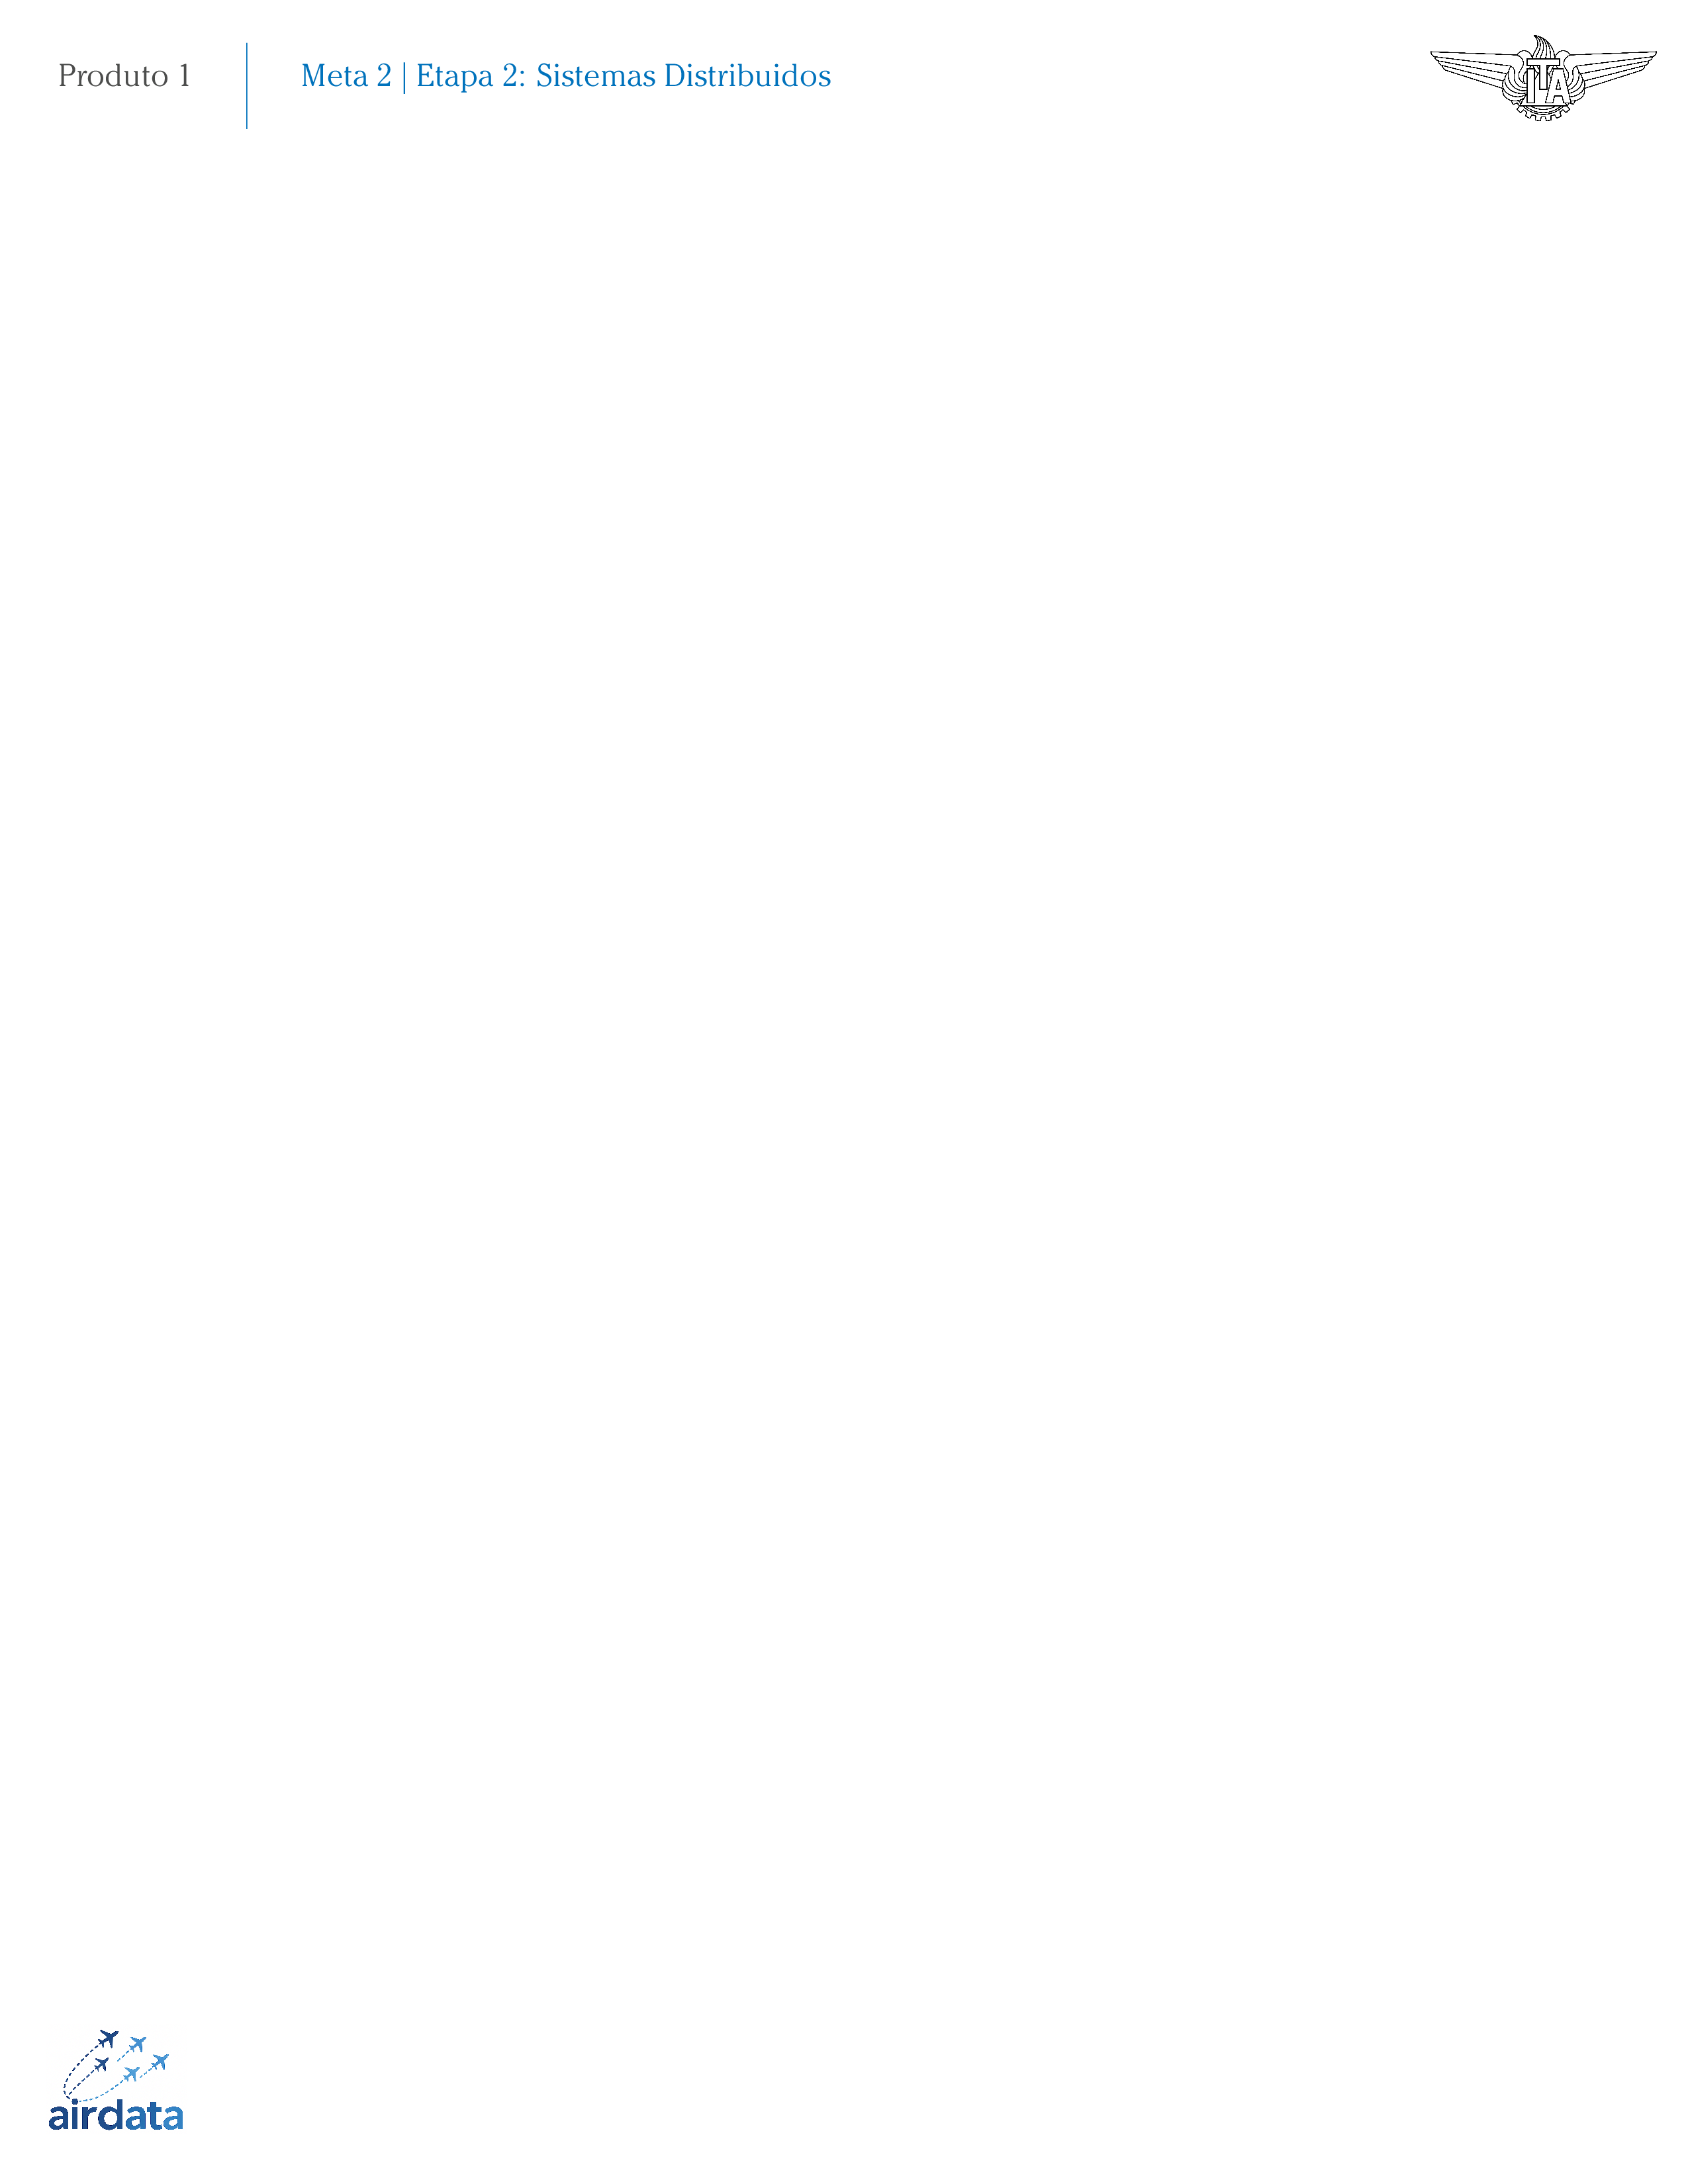
\includegraphics[width=\paperwidth,height=\paperheight]{capas/background.png}%
			\vfill
		}%
	}%
}

% Aplica a imagem de fundo em TODAS as páginas
\AddToShipoutPictureBG{\BackgroundPic}
      % marca d’água
% settings/pretextualpages.tex
% Define o background exclusivo para páginas pré-textuais

\newenvironment{pretextualblock}
{
	\ClearShipoutPictureBG
	\AddToShipoutPictureBG{
		\put(0,0){
			\parbox[b][\paperheight]{\paperwidth}{%
				
\includegraphics[width=\paperwidth,height=\paperheight]{capas/background_pretex}%
			}
		}
	}
}
{
	% settings/background.tex
% --- Imagem de fundo em todas as páginas ---

% Comando seguro para definir a imagem de fundo
\providecommand\BackgroundPic{%
	\put(0,0){%
		\parbox[b][\paperheight]{\paperwidth}{%
			\vfill
			\centering
			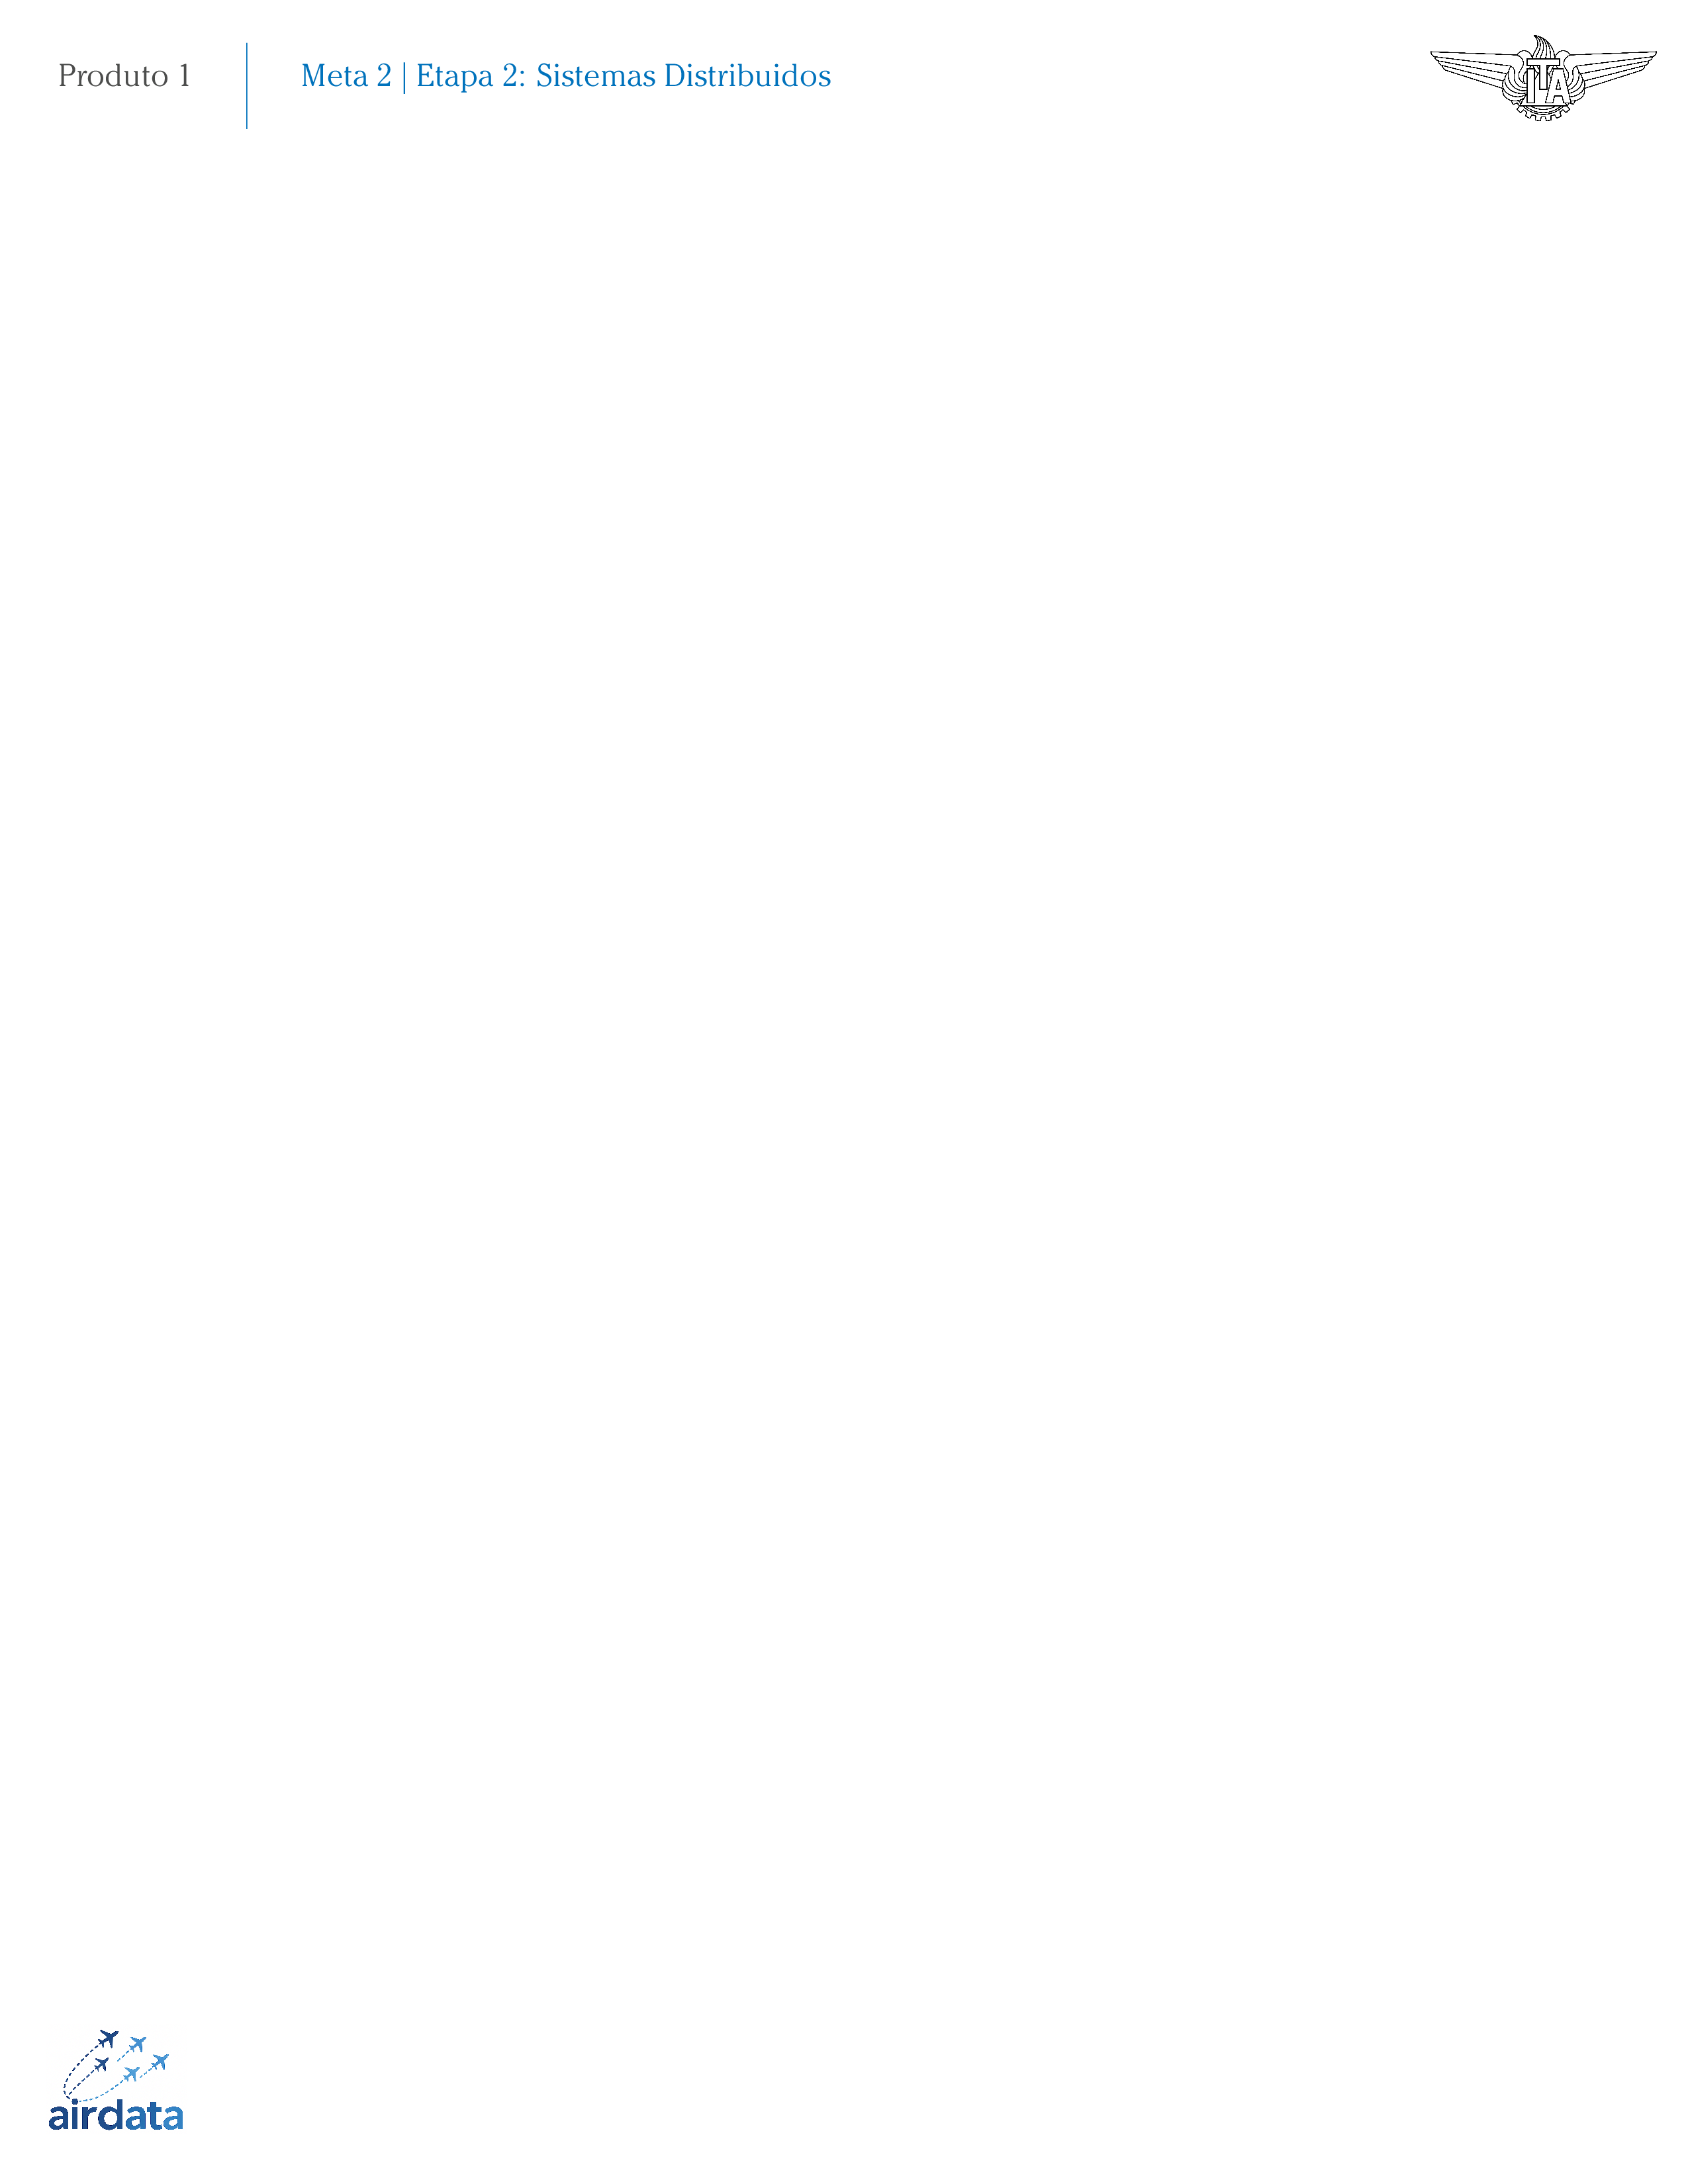
\includegraphics[width=\paperwidth,height=\paperheight]{capas/background.png}%
			\vfill
		}%
	}%
}

% Aplica a imagem de fundo em TODAS as páginas
\AddToShipoutPictureBG{\BackgroundPic}
 % Restaura o background padrão
}
 % sumário, listas etc.


\begin{document}
	
	%--------------------------------------------------------------------------
	% CAPA SEM NENHUMA NUMERAÇÃO
	%--------------------------------------------------------------------------
	\pagenumbering{gobble}
	
	% =======================================================================
	% === COVER PAGE GENERATION =============================================
	% =======================================================================
	% Cover is generated as PNG by: make generate-cover
	% To customize, edit variables in Makefile
	% -----------------------------------------------------------------------
	\makeDynamicCover
	% =======================================================================

	%--------------------------------------------------------------------------
	% PÁGINAS PRÉ-TEXTUAIS SEM NUMERAÇÃO
	%--------------------------------------------------------------------------
	\cleardoublepage
	\begingroup
	\pagenumbering{gobble}
	\pagestyle{empty}
	\begin{pretextualblock}
	
	
%--------------------------------------------------------------------------
% Histório de Versões
%--------------------------------------------------------------------------

\chapter*{Histórico de versões:}

	\begin{table}[H]
		\centering
		\begin{tabularx}{\textwidth}{|c|c|c|X|}
			\hline
			\textcolor{airdataBlue}{\textit{Versão}} &
			\textcolor{airdataBlue}{\textit{Data}} &
			\textcolor{airdataBlue}{\textit{Responsável}} &
			\textcolor{airdataBlue}{\textit{Descrição da alteração}} \\
			\hline
			\textcolor{gray}{1.0} & \textcolor{gray}{01/07/2025} & \textcolor{gray}{Prof. Dr.} & \textcolor{gray}{Versão inicial do produto X} \\
			\hline
			& & & \\
			\hline
			& & & \\
			\hline
		\end{tabularx}
	\end{table}


\newpage
\pagestyle{empty} 

%--------------------------------------------------------------------------	
% Coordenação Geral e de Etapa
%--------------------------------------------------------------------------	

\vspace*{2cm}    % funciona no topo da página
\begin{flushright}
	\textbf{Coordenação Geral}\\
	Prof. Dr. Cláudio Jorge Pinto Alves\\
	claudioj@ita.br\\
	\vspace*{10cm}
	\textbf{Gerente da Etapa}\\
	Prof. Dr. Elton Felipe Sbruzzi\\
	elton@ita.br
\end{flushright}

\newpage
\pagestyle{empty} 

%--------------------------------------------------------------------------
% Equipe ITA
%--------------------------------------------------------------------------	

\vspace*{2cm}    % funciona no topo da página
\begin{flushright}
	
	\textbf{Equipa ITA}\\
	\vspace*{1cm}
	
	Nome\\
	Função na Etapa\\
	\vspace*{1cm}
	
	Nome\\
	Função na Etapa\\
	\vspace*{1cm}
	
	Nome\\
	Função na Etapa\\
	\vspace*{1cm}

\end{flushright}


\newpage
\pagestyle{empty} 
%--------------------------------------------------------------------------	
% Descrição do Produto
%--------------------------------------------------------------------------	
\begin{flushleft}
	
\vspace*{15cm}	
\textcolor{airdataBlue}{\textbf{\LARGE Produto 1}}\\
\textcolor{airdataBlue}{Meta 2 \textbar{} Etapa 6: Tarifação}\\
\vspace*{5cm}	
Nome do Produto

\end{flushleft}
		
%--------------------------------------------------------------------------	
% Página em Branco
%--------------------------------------------------------------------------	
\newpage
\pagestyle{empty}      % remove visualmente número e cabeçalho
\textcolor{white}{Página de controle}
\newpage


\end{pretextualblock}
  % histórico de versões, equipe etc.
	\endgroup
	
	%--------------------------------------------------------------------------
	% CONTEÚDO COM NUMERAÇÃO ARÁBICA
	%--------------------------------------------------------------------------
	\cleardoublepage
	\pagenumbering{arabic}
	\setcounter{page}{1}
	\pagestyle{plain}
	
	%--------------------------------------------------------------------------
	% SUMÁRIO E LISTAS
	%--------------------------------------------------------------------------
	\tableofcontents
	
	\cleardoublepage
	
     \printglossary[type=\acronymtype, title=Lista de Siglas]

	
	\cleardoublepage
	\listoffigures
	
	\cleardoublepage
	\listoftables
	
	%--------------------------------------------------------------------------
	% CAPÍTULOS
	%--------------------------------------------------------------------------
	\cleardoublepage
	\pagestyle{plain}
	\chapter*{Sumário Executivo}
\addcontentsline{toc}{chapter}{Sumário Executivo}

O presente Produto faz parte da relação de entregas da Meta 2 Etapa 6 do TED --- Termo de Execução Descentralizada n.\ 1525720240005-003882/2024, firmado entre a Secretaria de Aviação Civil, cujo número de Processo é 50020.008564/2024-14. Tal TED foi decorrente de estruturação entre a SAC -- Secretaria de Aviação Civil e o ITA -- Instituto Tecnológico de Aeronáutica, com foco em ``Estudos para Aviação de Hoje e do Amanhã''. O ITA respondeu à demanda da SAC e o TED citado foi estruturado em 02 (duas) Metas com 16 (dezesseis) Etapas. O citado TED foi firmado no dia 20/12/2024.

\bigskip


% Opção 1: Usando minipage (Recomendada)
\textbf{Dados Referenciais:}
\begin{center}
	\begin{minipage}{0.6\textwidth}
		\raggedright
		TED n.\ 1525720240005-003882/2024\\
		Processo n.\ 50020.008564/2024-14\\
		Etapa XYZ da Meta kWM\\
		Produto XYZ\\
	\end{minipage}
\end{center}

\bigskip

Descrever, de forma rápida, o Produto que está sendo entregue. Texto aleatório.

\smallskip

Lorem ipsum dolor sit amet, consectetur adipiscing elit. Sed at erat venenatis, congue lorem vel, volutpat diam. Quisque ac tempus nisi...


\gls{fab} testando.
	
	\cleardoublepage
	\pagestyle{plain}
	\chapter{Introdução ao Template TED ITA-SAC}

Este manual documenta o uso e as boas práticas associadas ao \textbf{Template ITA-SAC}, desenvolvido no contexto do projeto Estudos para a Aviação de Hoje e do Amanhã. O template foi concebido para garantir padronização, qualidade visual e conformidade com as normas técnicas e científicas exigidas em relatórios e entregas institucionais.

O modelo está implementado em \LaTeX, com modularização completa para facilitar a manutenção, customização e reuso por diferentes autores. A compilação deve ser feita utilizando o motor \texttt{XeLaTeX}, pois o sistema de fontes depende do pacote \texttt{fontspec}, utilizado para habilitar a tipografia oficial do projeto (Cheltenham ITC Pro).

\vspace{1em}

\textbf{Principais características do template:}
\begin{itemize}
    \item Estrutura modular com arquivos separados para capa, plano de fundo, layout, fontes, cores e títulos;
    \item Compatível com normas da ABNT (\texttt{abntex2cite});
    \item Fonte principal: \textbf{Cheltenham ITC Pro}, via XeLaTeX;
    \item Estilo visual limpo e profissional, com suporte a capa institucional e marca d’água;
    \item Compilação automatizada via \texttt{Makefile};
    \item Pronto para inclusão de capítulos, glossários, siglas e bibliografia.
\end{itemize}

\vspace{1em}

\textbf{Estrutura de diretórios:}

\begin{verbatim}
	.
	|- main.tex                 % Arquivo principal
	|- settings/                % Configurações gerais
	|  |- background.tex        % Marca d’água e fundo
	|  |- coverpage.tex         % Página de capa
	|  |- fonts.tex             % Fonte Cheltenham
	|  |- ...
	|- caps/                    % Capítulos do relatório
	|- Makefile                 % Automação
\end{verbatim}

Este documento é dividido em capítulos, cada um explicando um aspecto do template, para que os autores possam modificar e estender com segurança, mantendo a padronização do projeto Estudos para a Aviação de Hoje e do Amanhã.



	
	\cleardoublepage
	\pagestyle{plain}
	\chapter{Requisitos e Instalação}

Este capítulo apresenta os requisitos técnicos para compilar e personalizar o \textbf{Template TED ITA-SAC}, bem como orientações de instalação em diferentes ambientes.

\section{Ambiente recomendado}

O template foi testado e validado em:
\begin{itemize}
    \item \textbf{Distribuição \LaTeX:} TeX Live 2023 ou superior (recomendado: TeX Live 2025);
    \item \textbf{Compilador:} XeLaTeX (\texttt{xelatex});
    \item \textbf{Editor:} TeXstudio, VSCode + LaTeX Workshop, Overleaf (parcial).
\end{itemize}

\section{Instalação no Linux (TeX Live)}

Para usuários Linux (ex: Ubuntu), recomenda-se a instalação do TeX Live completo:

\begin{verbatim}
sudo apt update
sudo apt install texlive-full
\end{verbatim}

Caso deseje controle via \texttt{tlmgr}, instale a versão mais recente diretamente do site da TeX Live:
\url{https://www.tug.org/texlive/acquire-netinstall.html}

\section{Instalação de fontes (Cheltenham ITC Pro)}

A fonte \textbf{Cheltenham ITC Pro} deve estar instalada no sistema operacional. Copie os arquivos \texttt{.otf} para o diretório de fontes do sistema (exemplo para Linux):

\begin{verbatim}
mkdir -p ~/.fonts/cheltenham
cp *.otf ~/.fonts/cheltenham/
fc-cache -fv
\end{verbatim}

No Windows, clique com o botão direito nos arquivos \texttt{.otf} e escolha \textit{"Instalar"}.

\section{Compilação com Makefile (recomendado)}

A compilação automática pode ser feita via \texttt{make}, no terminal, a partir do diretório do projeto:

\begin{verbatim}
make
\end{verbatim}

Esse comando realiza:
\begin{enumerate}
    \item Compilação com XeLaTeX;
    \item Geração de glossário (se ativado);
    \item Execução do BibTeX;
    \item Duas recompilações para acerto de referências.
\end{enumerate}

\section{Uso no Overleaf}

Para uso online:
\begin{itemize}
    \item A compilação deve ser configurada como XeLaTeX;
    \item Os arquivos de fonte \texttt{.otf} devem ser enviados ao projeto;
    \item O glossário (se usado) pode exigir configuração especial;
    \item Limitações podem ocorrer em pacotes como \texttt{background} ou \texttt{shell-escape}.
\end{itemize}

\section{Pacotes adicionais recomendados}

Certifique-se de que os seguintes pacotes estejam disponíveis:

\begin{itemize}
    \item \texttt{fontspec, xcolor, background, titlesec}
    \item \texttt{abntex2cite, glossaries-extra, biblatex, makeindex}
    \item \texttt{geometry, fancyhdr, enumitem, graphicx, hyperref}
\end{itemize}

Para instalar manualmente via \texttt{tlmgr}:

\begin{verbatim}
tlmgr install glossaries-extra abntex2cite background titlesec
\end{verbatim}



	
	
	\cleardoublepage
	\pagestyle{plain}
	\chapter{Estrutura do Template}

O template TED ITA-SAC foi organizado de forma modular, para facilitar manutenção, reuso e colaboração entre diferentes autores. A estrutura principal está organizada da seguinte forma:

\section{Visão geral}

\begin{verbatim}
	.
	|- main.tex                 % Arquivo principal (documento raiz)
	|- settings/                % Configurações gerais
	|  |- background.tex        % Marca d’água e fundo
	|  |- coverpage.tex         % Página de capa
	|  |- fonts.tex             % Fonte Cheltenham
	|  |- pretextualpages.tex  % Sumário, listas, elementos iniciais
	|  |- setabnt.tex          % Estilo de citação ABNT
	|  |- setcolor.tex         % Paleta de cores do template
	|  |- setlayout.tex        % Margens, espaçamento, cabeçalho
	|  |- settitles.tex        % Estilo de títulos e capítulos
	|  \_ usepackage.tex       % Pacotes utilizados no projeto
	|- caps/                   % Capítulos do relatório
	|  |- cap00.tex            % Introdução
	|  |- cap01.tex            % Conteúdo específico
	|  \_ etc.
	|- siglas/                 % (Opcional) Siglas, glossários
	|- refs/                   % (Opcional) Arquivos .bib
	\_ Makefile                % Automação de compilação
\end{verbatim}


\section{Função de cada componente}

\begin{itemize}
    \item \texttt{main.tex}: ponto de entrada do projeto. Controla a ordem dos elementos.
    \item \texttt{settings/}: conjunto de arquivos para configurar todos os aspectos do template.
    \item \texttt{caps/}: contém os capítulos do relatório (modularizados).
    \item \texttt{siglas/}: pasta destinada ao glossário e acrônimos, caso ativado.
    \item \texttt{refs/}: local sugerido para o arquivo de bibliografia (\texttt{.bib}).
    \item \texttt{Makefile}: automatiza as etapas de compilação (XeLaTeX + BibTeX + Glossário).
\end{itemize}

\section{Ordem de carregamento no \texttt{main.tex}}

O arquivo \texttt{main.tex} importa os componentes da seguinte forma:

\begin{verbatim}
% defs_setusepackage.tex
% --- PACOTES DO TEMPLATE AIRDATA ---


% --- Tipografia e fontes ---
\usepackage{fontspec}       % Uso de fontes OpenType com XeLaTeX

% --- Cores institucionais ---
\usepackage{xcolor}         % Suporte a cores em HTML, RGB etc.

% --- Gráficos e imagens ---
\usepackage{graphicx}       % Inclusão de imagens (.png, .pdf etc.)
\usepackage{eso-pic}        % Permite inserir elementos em todas as páginas (fundo, logos)

% --- Formatação e layout ---

\usepackage{fancyhdr}       % Cabeçalho e rodapé customizados
\usepackage{titlesec}       % Personalização de títulos (\chapter, \section etc.)

% --- Tabelas ---
\usepackage{array}
\usepackage{booktabs}
\usepackage{float}
\usepackage{tabularx}

\usepackage[acronym]{glossaries-extra}
\setabbreviationstyle[acronym]{long-short}
\makeglossaries


% Pacotes ABNT
\usepackage[alf]{abntex2cite}  % ou [num] para numérico
% settings/setabnt.tex
% --- Configurações gerais para padrão ABNT (relatórios acadêmicos) ---

% --------------------------
% Idioma
% --------------------------
\usepackage{polyglossia}
\setdefaultlanguage{portuguese}


% --------------------------
% Margens ABNT (NBR 14724)
% Esquerda e superior: 3 cm | Direita e inferior: 2 cm
% --------------------------
\usepackage[a4paper,top=3cm,bottom=2cm,left=3cm,right=2cm]{geometry}

% --------------------------
% Espaçamento entre linhas (1.5) — ABNT exige entre 1.5 e 2.0
% --------------------------
\usepackage{setspace}
\onehalfspacing

% --------------------------
% Espaçamento entre parágrafos: nenhum (ABNT)
% Recuo da primeira linha de cada parágrafo (1.25 cm recomendado)
% --------------------------

\setlength{\parindent}{0pt}   % Remove o recuo de parágrafos
\setlength{\parskip}{1em}     % Adiciona espaço entre parágrafos (opcional)

% settings/setlayout.tex
% --- Configuração de layout de página e numeração ---

\usepackage{fancyhdr}
\pagestyle{fancy}

\fancyhf{}                    % Limpa cabeçalho e rodapé
\fancyfoot[R]{\thepage}       % Número da página no canto inferior direito
\renewcommand{\headrulewidth}{0pt} % Remove linha superior
\renewcommand{\footrulewidth}{0pt} % Remove linha inferior
\setlength{\footskip}{30pt}   % Espaço do rodapé

% Aplica o mesmo layout à página de abertura dos capítulos
\fancypagestyle{plain}{%
	\fancyhf{}
	\fancyfoot[R]{\thepage}
	\renewcommand{\headrulewidth}{0pt}
	\renewcommand{\footrulewidth}{0pt}
}

% defs_fonts.tex
% --- Fontes utilizadas no template AIRDATA ---

% Define a fonte principal do documento
\setmainfont{CheltenhamITCPro-Book}[
Path = ./fonts/,
Extension = .otf,
ItalicFont = CheltenhamITCPro-BookItalic,
BoldFont = CheltenhamITCPro-Bold,
BoldItalicFont = CheltenhamITCPro-BoldItalic
]

% Define a fonte "Light" como comando \useFontLight
\newfontfamily\useFontLight{CheltenhamITCPro-Light}[
Path = ./fonts/,
Extension = .otf,
ItalicFont = CheltenhamITCPro-LightItalic
]

% Define a fonte "Ultra" como comando \useFontUltra
\newfontfamily\useFontUltra{CheltenhamITCPro-Ultra}[
Path = ./fonts/,
Extension = .otf,
ItalicFont = CheltenhamITCPro-UltraItalic
]


\providecommand{\useFontLight}{}
\providecommand{\useFontUltra}{}

% settings/setcolor.tex
% --- Definições de cores do projeto AIRDATA ---

% Importante: não utilize o comando \usepackage{xcolor} aqui.
% Esse pacote já está carregado no arquivo settings/usepackage.tex.

% Cor azul institucional AIRDATA
\definecolor{airdataBlue}{HTML}{2f84c6}

% ========================================
% PALETA DE CORES - METAS E ETAPAS
% ========================================

% Cores de Coordenação
\definecolor{coordMeta1}{HTML}{272a6a}
\definecolor{coordMeta2}{HTML}{388fcd}

% --- META 1 ---
\definecolor{meta1etapa1}{HTML}{283880}
\definecolor{meta1etapa2}{HTML}{204196}
\definecolor{meta1etapa3}{HTML}{2451a4}
\definecolor{meta1etapa4}{HTML}{2b61ae}
\definecolor{meta1etapa5}{HTML}{2d72ba}
\definecolor{meta1etapa6}{HTML}{2f84c6}

% --- META 2 ---
\definecolor{meta2etapa1}{HTML}{388fcd}
\definecolor{meta2etapa2}{HTML}{6597ca}
\definecolor{meta2etapa3}{HTML}{6392bd}
\definecolor{meta2etapa4}{HTML}{618eb1}
\definecolor{meta2etapa5}{HTML}{5e89a7}
\definecolor{meta2etapa6}{HTML}{5c859c}
\definecolor{meta2etapa7}{HTML}{4d7d94}
\definecolor{meta2etapa8}{HTML}{3f738b}
\definecolor{meta2etapa9}{HTML}{306983}
\definecolor{meta2etapa10}{HTML}{215f7b}

% ========================================
% CORES ESPECIAIS PARA CAPAS
% ========================================

% Cor creme para fundo de capa (conforme feedback ChatGPT)
\definecolor{creamBg}{RGB}{250,245,225}

% ========================================
% COR PRINCIPAL DO PROJETO
% ========================================

% Cor principal do projeto (Meta 2 Etapa 6 por padrão)
% Esta cor é usada para destacar o projeto atual na paleta
\definecolor{projectMainColor}{named}{meta2etapa6}

% settings/settitles.tex
% --- Estilo e formatação dos títulos do template AIRDATA ---

\RequirePackage{titlesec}

% Mostra a numeração até subsubsection
\setcounter{secnumdepth}{3}

% -------------------------------
% CAPÍTULO (CHAPTER) — 16 pt, azul, normal
% -------------------------------
\titleformat{\chapter}[hang]
{\color{airdataBlue}\normalfont\fontsize{16}{20}\selectfont}
{\thechapter}{1em}{}

% -------------------------------
% SEÇÃO (SECTION) — 14 pt, azul, itálico
% -------------------------------
\titleformat{\section}
{\color{airdataBlue}\normalfont\fontsize{14}{18}\selectfont}
{\thesection}{1em}{}

% -------------------------------
% SUBSEÇÃO (SUBSECTION) — 14 pt, azul, itálico
% -------------------------------
\titleformat{\subsection}
{\color{airdataBlue}\normalfont\itshape\fontsize{14}{17}\selectfont}
{\thesubsection}{1em}{}

% -------------------------------
% SUBSUBSEÇÃO (SUBSUBSECTION) — 12 pt, azul, itálico
% -------------------------------
\titleformat{\subsubsection}
{\color{airdataBlue}\normalfont\itshape\fontsize{12}{14}\selectfont}
{\thesubsubsection}{1em}{}

% -------------------------------
% Espaçamento vertical entre título e texto
% -------------------------------
\titlespacing*{\chapter}      {0pt}{20pt plus 2pt}{10pt plus 2pt}
\titlespacing*{\section}      {0pt}{16pt plus 2pt}{8pt plus 2pt}
\titlespacing*{\subsection}   {0pt}{14pt plus 2pt}{6pt plus 2pt}
\titlespacing*{\subsubsection}{0pt}{12pt plus 2pt}{4pt plus 2pt}

% settings/coverpage.tex
% --- Capa com imagem de fundo ocupando toda a página ---

\newcommand\makecover{
	\ClearShipoutPictureBG  % remove o background institucional temporariamente
	\AddToShipoutPicture*{
		\put(0,0){
			
\includegraphics[width=\paperwidth,height=\paperheight]{capas/cover.png}
		}
	}
	\begin{titlepage}
		\null  % necessário para forçar a renderização da imagem
		\thispagestyle{empty}
		\newpage
	\end{titlepage}
	\ClearShipoutPictureBG  % limpa a capa para evitar efeito nas próximas páginas
	\AddToShipoutPictureBG{\BackgroundPic}  % restaura o background institucional
}

% settings/background.tex
% --- Imagem de fundo em todas as páginas ---

% Comando seguro para definir a imagem de fundo
\providecommand\BackgroundPic{%
	\put(0,0){%
		\parbox[b][\paperheight]{\paperwidth}{%
			\vfill
			\centering
			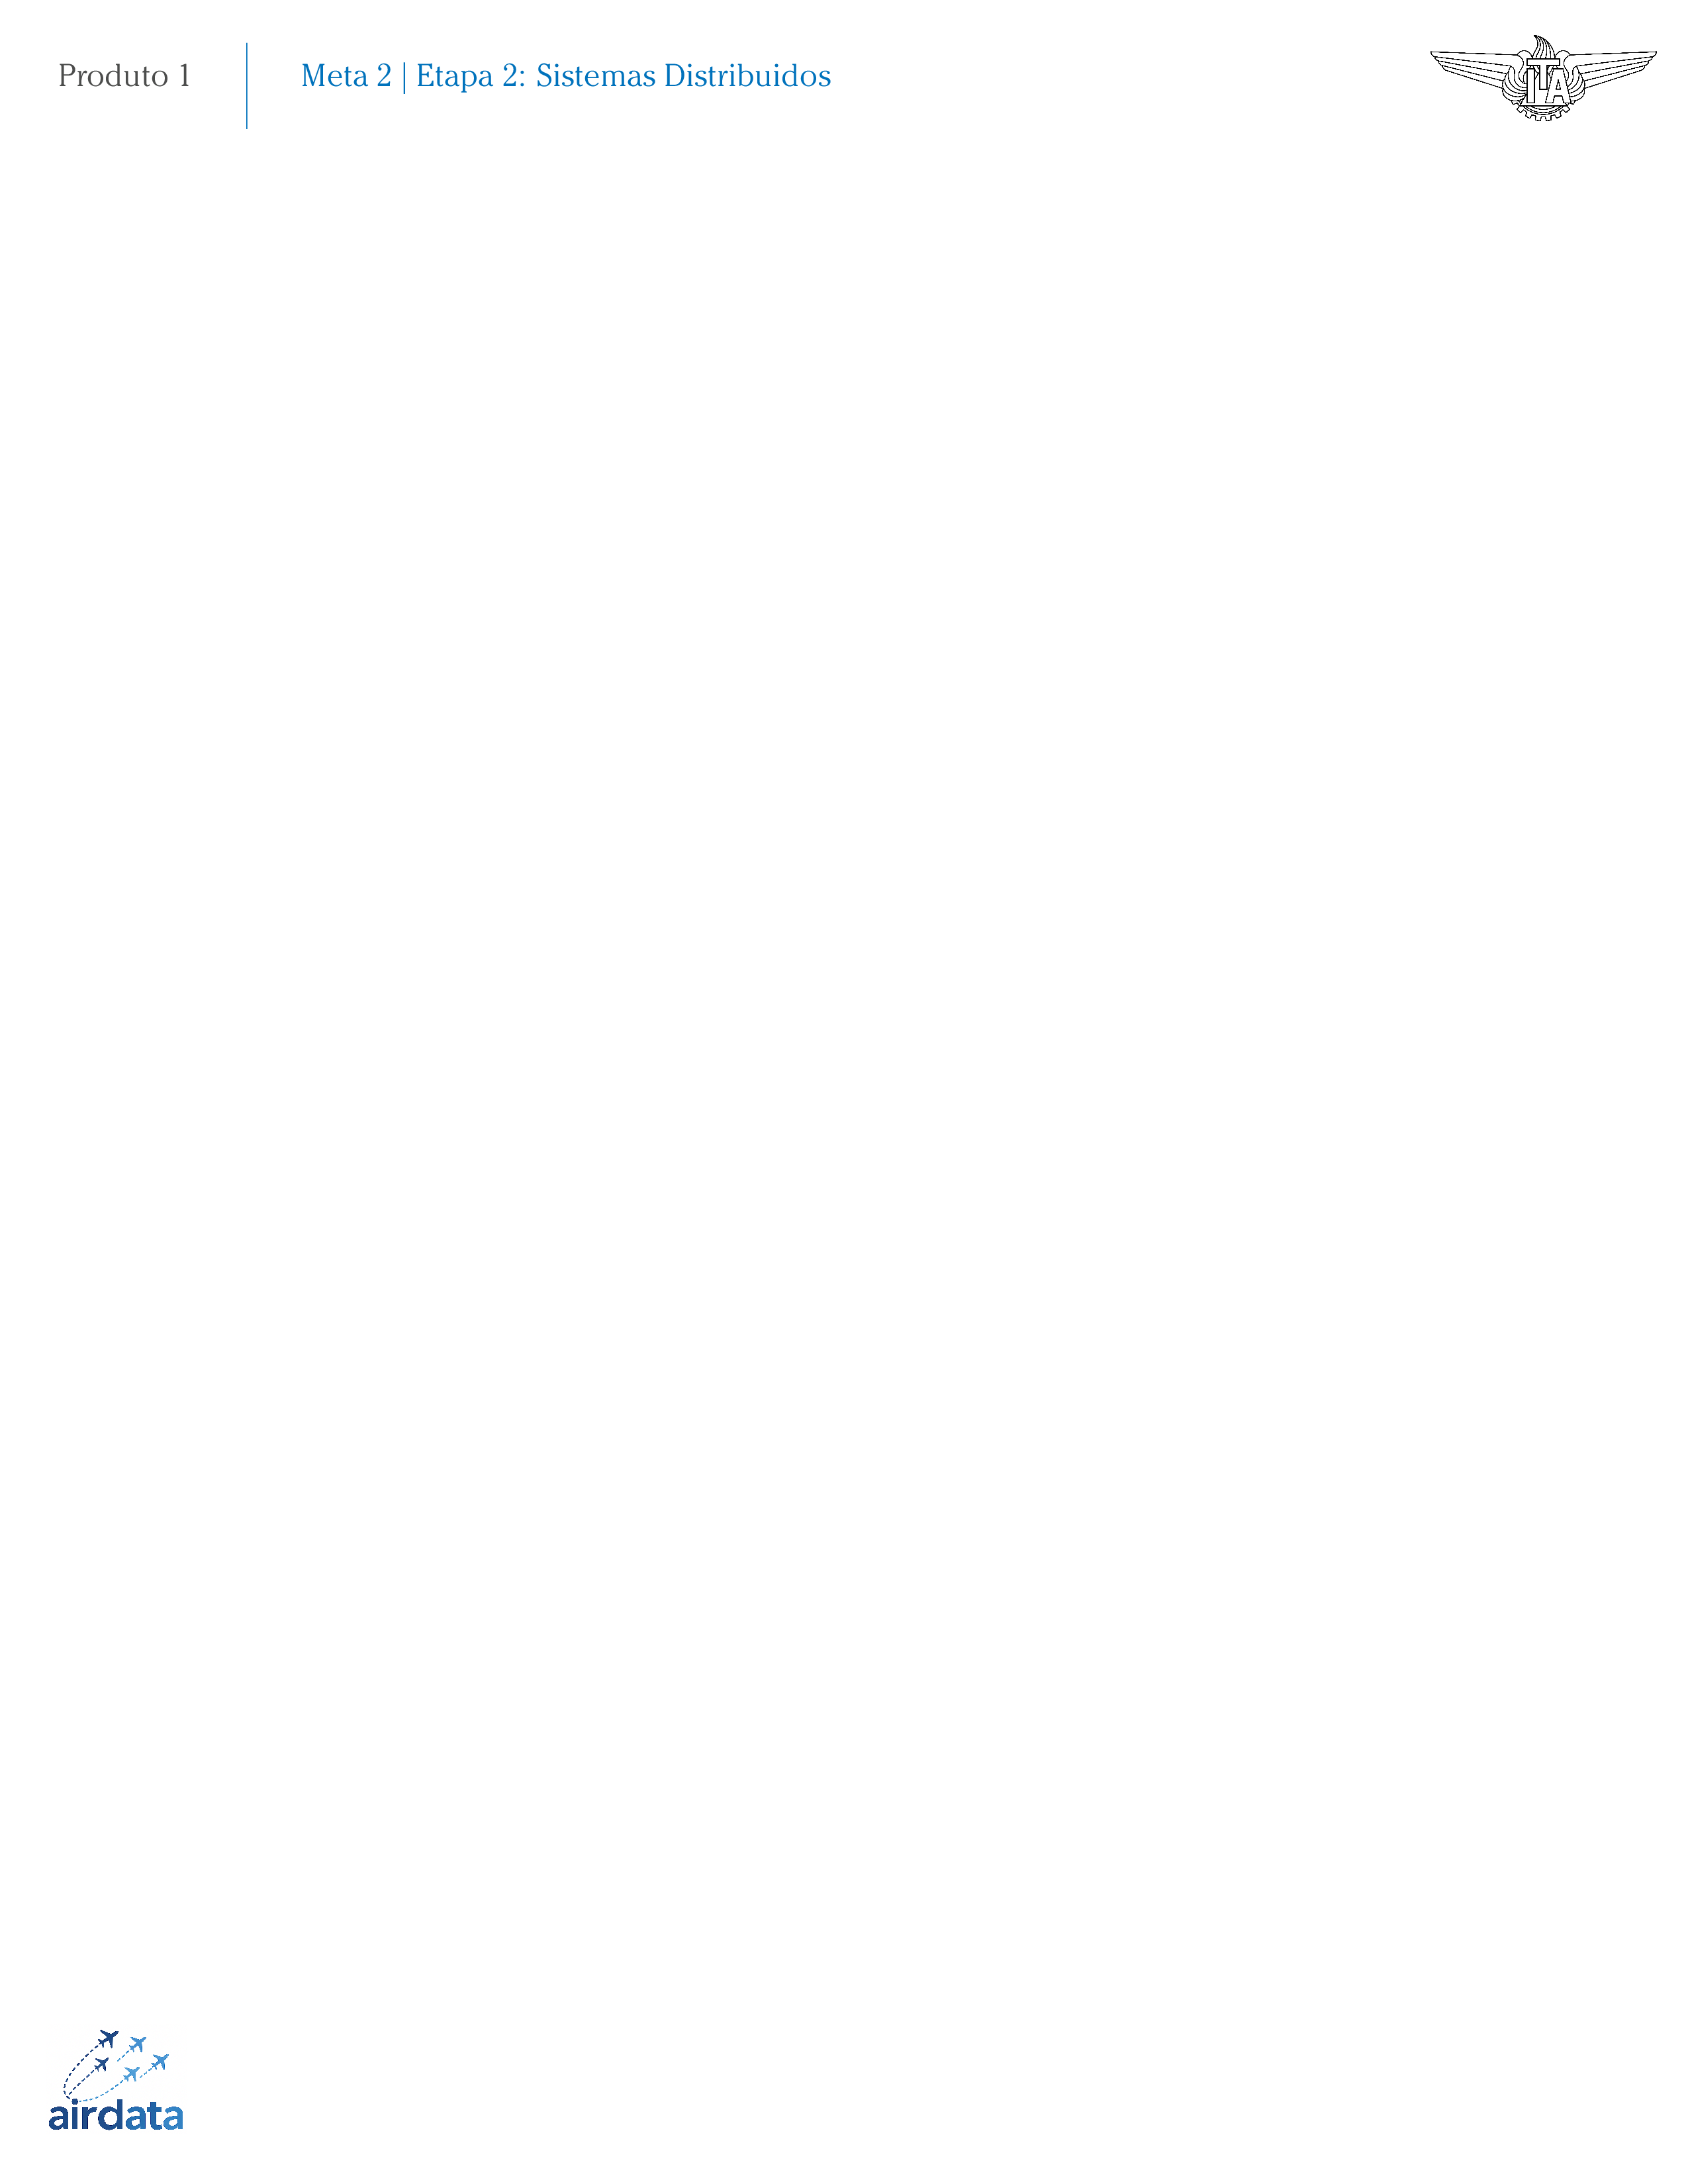
\includegraphics[width=\paperwidth,height=\paperheight]{capas/background.png}%
			\vfill
		}%
	}%
}

% Aplica a imagem de fundo em TODAS as páginas
\AddToShipoutPictureBG{\BackgroundPic}

% settings/pretextualpages.tex
% Define o background exclusivo para páginas pré-textuais

\newenvironment{pretextualblock}
{
	\ClearShipoutPictureBG
	\AddToShipoutPictureBG{
		\put(0,0){
			\parbox[b][\paperheight]{\paperwidth}{%
				
\includegraphics[width=\paperwidth,height=\paperheight]{capas/background_pretex}%
			}
		}
	}
}
{
	% settings/background.tex
% --- Imagem de fundo em todas as páginas ---

% Comando seguro para definir a imagem de fundo
\providecommand\BackgroundPic{%
	\put(0,0){%
		\parbox[b][\paperheight]{\paperwidth}{%
			\vfill
			\centering
			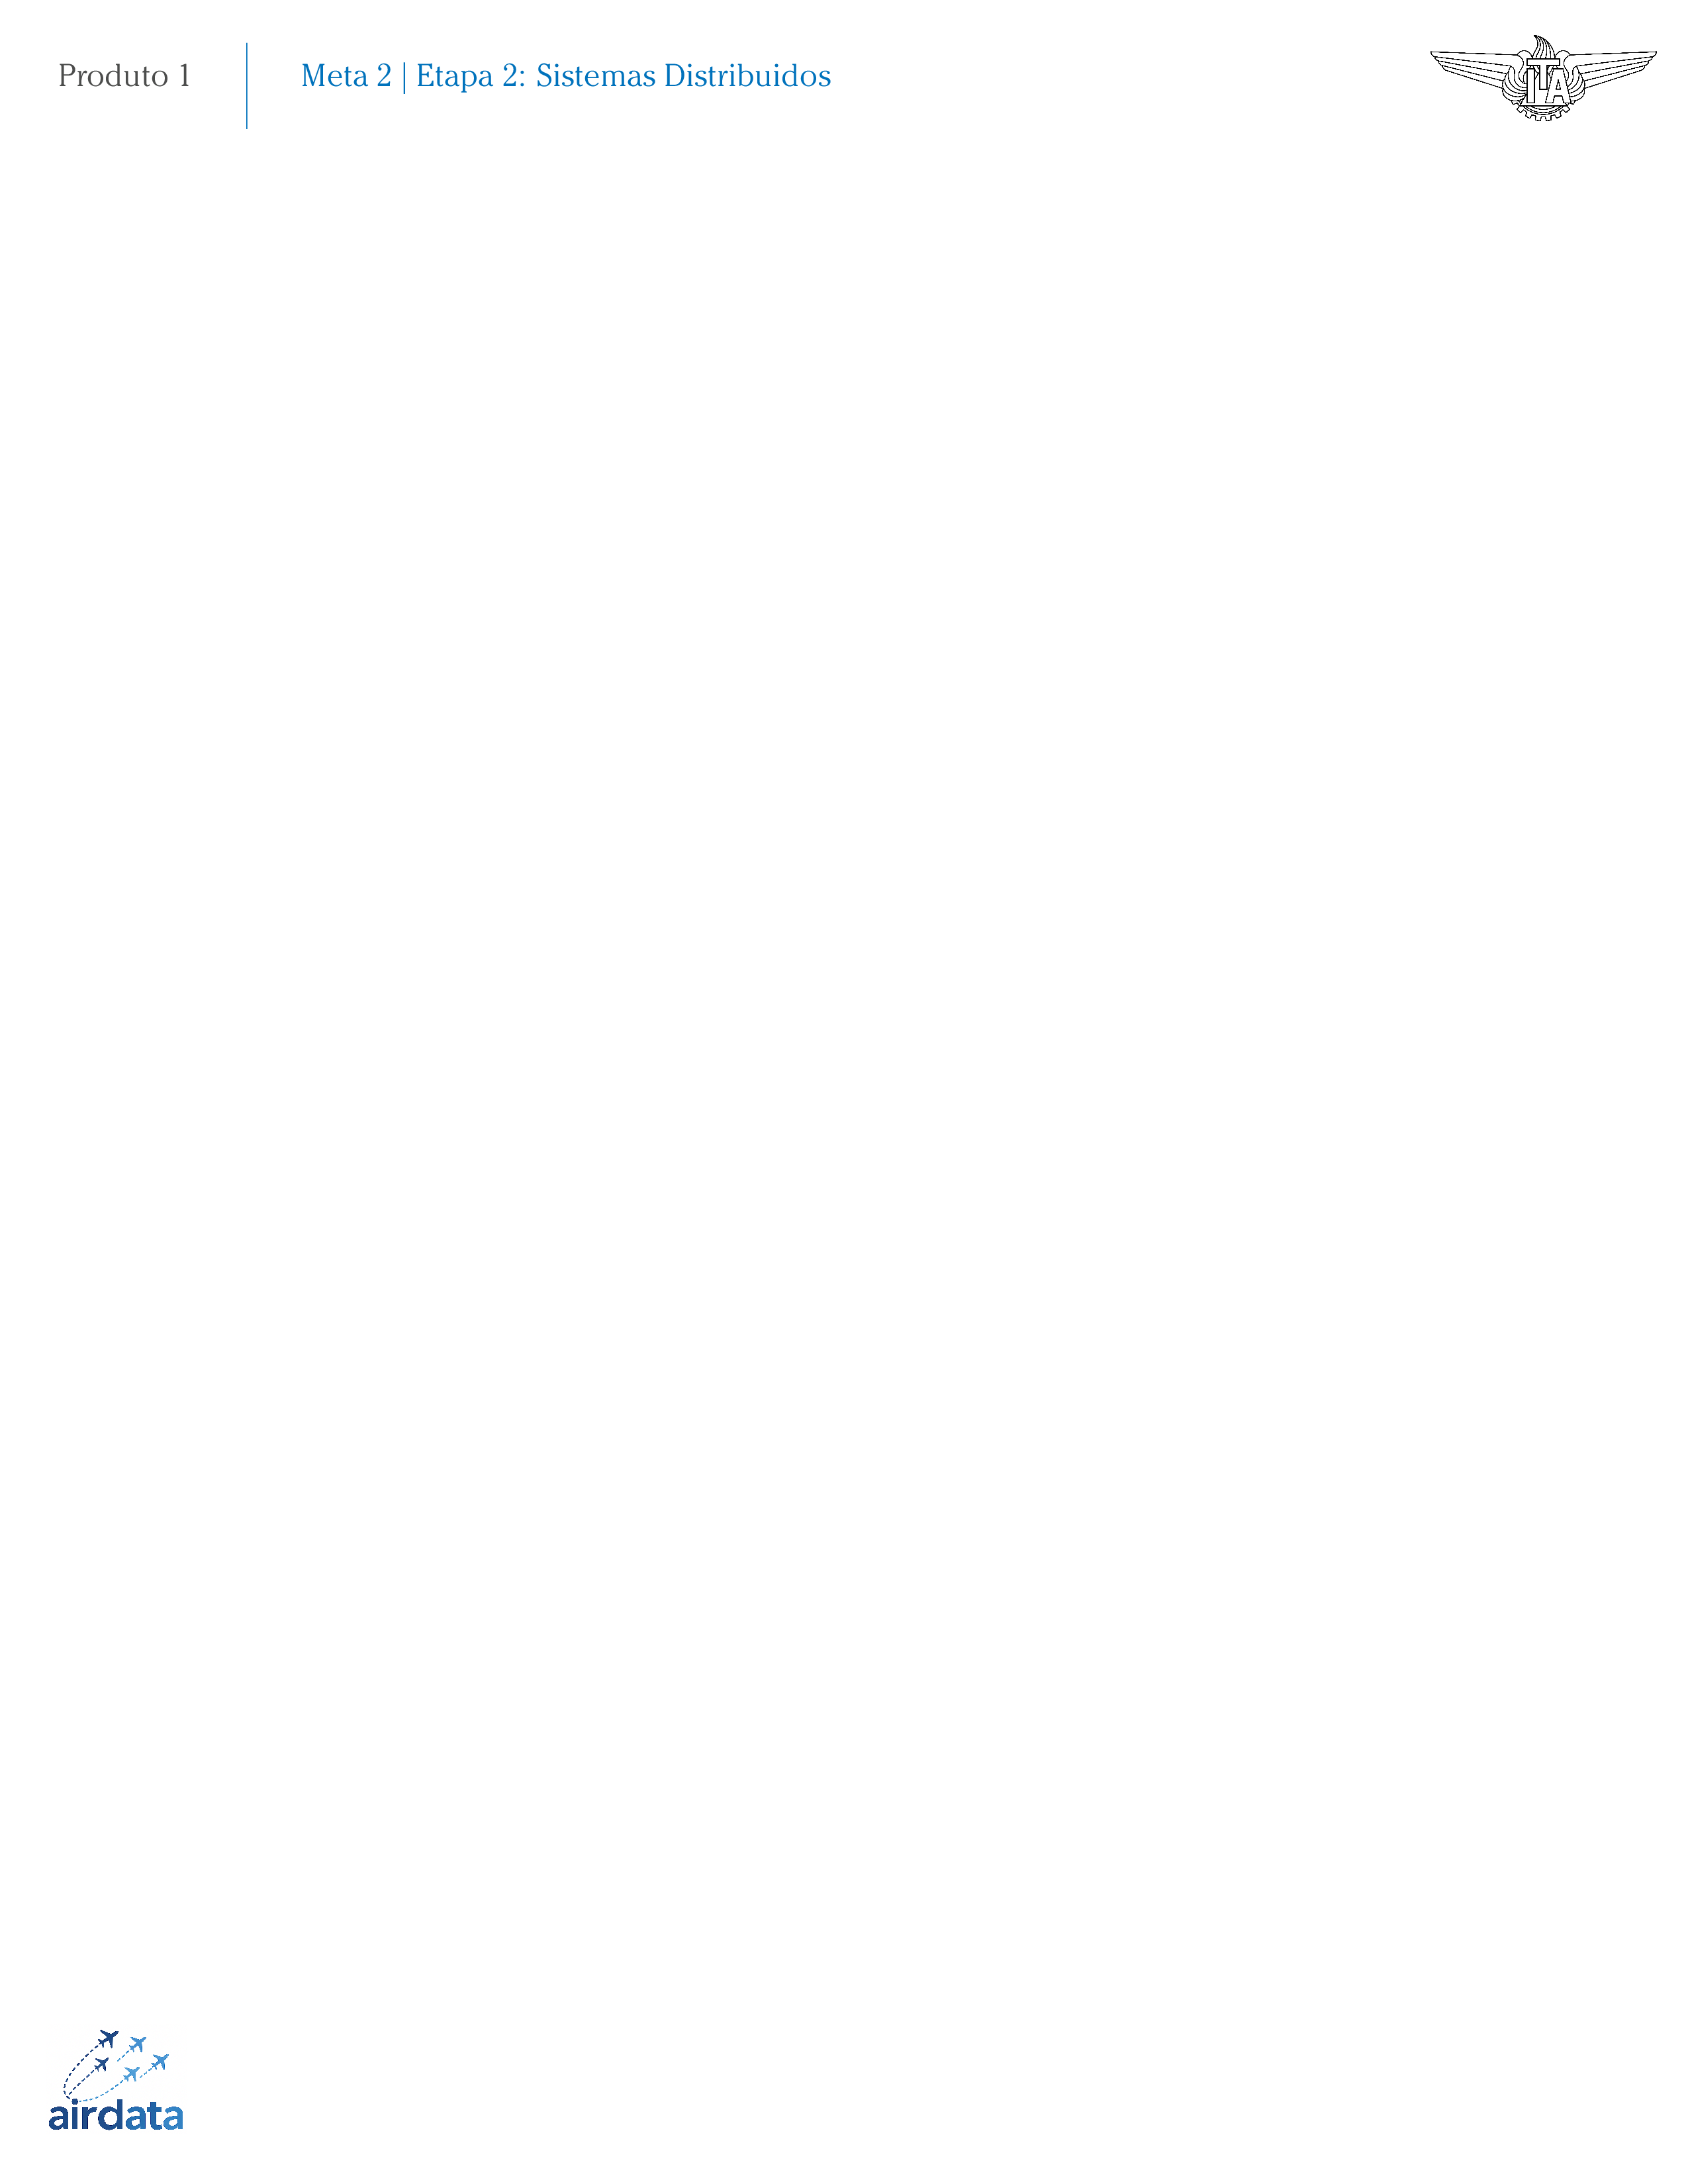
\includegraphics[width=\paperwidth,height=\paperheight]{capas/background.png}%
			\vfill
		}%
	}%
}

% Aplica a imagem de fundo em TODAS as páginas
\AddToShipoutPictureBG{\BackgroundPic}
 % Restaura o background padrão
}

\end{verbatim}

Essa ordem é proposital para garantir que os pacotes e estilos sejam carregados antes dos elementos visuais como capa e plano de fundo.

\section{Sugestão de novos capítulos}

Novos arquivos podem ser adicionados à pasta \texttt{caps/} com nomes como \texttt{cap03.tex}, \texttt{cap04.tex}, etc. A inclusão no documento é feita via:

\begin{verbatim}
\chapter{Estrutura do Template}

O template TED ITA-SAC foi organizado de forma modular, para facilitar manutenção, reuso e colaboração entre diferentes autores. A estrutura principal está organizada da seguinte forma:

\section{Visão geral}

\begin{verbatim}
	.
	|- main.tex                 % Arquivo principal (documento raiz)
	|- settings/                % Configurações gerais
	|  |- background.tex        % Marca d’água e fundo
	|  |- coverpage.tex         % Página de capa
	|  |- fonts.tex             % Fonte Cheltenham
	|  |- pretextualpages.tex  % Sumário, listas, elementos iniciais
	|  |- setabnt.tex          % Estilo de citação ABNT
	|  |- setcolor.tex         % Paleta de cores do template
	|  |- setlayout.tex        % Margens, espaçamento, cabeçalho
	|  |- settitles.tex        % Estilo de títulos e capítulos
	|  \_ usepackage.tex       % Pacotes utilizados no projeto
	|- caps/                   % Capítulos do relatório
	|  |- cap00.tex            % Introdução
	|  |- cap01.tex            % Conteúdo específico
	|  \_ etc.
	|- siglas/                 % (Opcional) Siglas, glossários
	|- refs/                   % (Opcional) Arquivos .bib
	\_ Makefile                % Automação de compilação
\end{verbatim}


\section{Função de cada componente}

\begin{itemize}
    \item \texttt{main.tex}: ponto de entrada do projeto. Controla a ordem dos elementos.
    \item \texttt{settings/}: conjunto de arquivos para configurar todos os aspectos do template.
    \item \texttt{caps/}: contém os capítulos do relatório (modularizados).
    \item \texttt{siglas/}: pasta destinada ao glossário e acrônimos, caso ativado.
    \item \texttt{refs/}: local sugerido para o arquivo de bibliografia (\texttt{.bib}).
    \item \texttt{Makefile}: automatiza as etapas de compilação (XeLaTeX + BibTeX + Glossário).
\end{itemize}

\section{Ordem de carregamento no \texttt{main.tex}}

O arquivo \texttt{main.tex} importa os componentes da seguinte forma:

\begin{verbatim}
% defs_setusepackage.tex
% --- PACOTES DO TEMPLATE AIRDATA ---


% --- Tipografia e fontes ---
\usepackage{fontspec}       % Uso de fontes OpenType com XeLaTeX

% --- Cores institucionais ---
\usepackage{xcolor}         % Suporte a cores em HTML, RGB etc.

% --- Gráficos e imagens ---
\usepackage{graphicx}       % Inclusão de imagens (.png, .pdf etc.)
\usepackage{eso-pic}        % Permite inserir elementos em todas as páginas (fundo, logos)

% --- Formatação e layout ---

\usepackage{fancyhdr}       % Cabeçalho e rodapé customizados
\usepackage{titlesec}       % Personalização de títulos (\chapter, \section etc.)

% --- Tabelas ---
\usepackage{array}
\usepackage{booktabs}
\usepackage{float}
\usepackage{tabularx}

\usepackage[acronym]{glossaries-extra}
\setabbreviationstyle[acronym]{long-short}
\makeglossaries


% Pacotes ABNT
\usepackage[alf]{abntex2cite}  % ou [num] para numérico
% settings/setabnt.tex
% --- Configurações gerais para padrão ABNT (relatórios acadêmicos) ---

% --------------------------
% Idioma
% --------------------------
\usepackage{polyglossia}
\setdefaultlanguage{portuguese}


% --------------------------
% Margens ABNT (NBR 14724)
% Esquerda e superior: 3 cm | Direita e inferior: 2 cm
% --------------------------
\usepackage[a4paper,top=3cm,bottom=2cm,left=3cm,right=2cm]{geometry}

% --------------------------
% Espaçamento entre linhas (1.5) — ABNT exige entre 1.5 e 2.0
% --------------------------
\usepackage{setspace}
\onehalfspacing

% --------------------------
% Espaçamento entre parágrafos: nenhum (ABNT)
% Recuo da primeira linha de cada parágrafo (1.25 cm recomendado)
% --------------------------

\setlength{\parindent}{0pt}   % Remove o recuo de parágrafos
\setlength{\parskip}{1em}     % Adiciona espaço entre parágrafos (opcional)

% settings/setlayout.tex
% --- Configuração de layout de página e numeração ---

\usepackage{fancyhdr}
\pagestyle{fancy}

\fancyhf{}                    % Limpa cabeçalho e rodapé
\fancyfoot[R]{\thepage}       % Número da página no canto inferior direito
\renewcommand{\headrulewidth}{0pt} % Remove linha superior
\renewcommand{\footrulewidth}{0pt} % Remove linha inferior
\setlength{\footskip}{30pt}   % Espaço do rodapé

% Aplica o mesmo layout à página de abertura dos capítulos
\fancypagestyle{plain}{%
	\fancyhf{}
	\fancyfoot[R]{\thepage}
	\renewcommand{\headrulewidth}{0pt}
	\renewcommand{\footrulewidth}{0pt}
}

% defs_fonts.tex
% --- Fontes utilizadas no template AIRDATA ---

% Define a fonte principal do documento
\setmainfont{CheltenhamITCPro-Book}[
Path = ./fonts/,
Extension = .otf,
ItalicFont = CheltenhamITCPro-BookItalic,
BoldFont = CheltenhamITCPro-Bold,
BoldItalicFont = CheltenhamITCPro-BoldItalic
]

% Define a fonte "Light" como comando \useFontLight
\newfontfamily\useFontLight{CheltenhamITCPro-Light}[
Path = ./fonts/,
Extension = .otf,
ItalicFont = CheltenhamITCPro-LightItalic
]

% Define a fonte "Ultra" como comando \useFontUltra
\newfontfamily\useFontUltra{CheltenhamITCPro-Ultra}[
Path = ./fonts/,
Extension = .otf,
ItalicFont = CheltenhamITCPro-UltraItalic
]


\providecommand{\useFontLight}{}
\providecommand{\useFontUltra}{}

% settings/setcolor.tex
% --- Definições de cores do projeto AIRDATA ---

% Importante: não utilize o comando \usepackage{xcolor} aqui.
% Esse pacote já está carregado no arquivo settings/usepackage.tex.

% Cor azul institucional AIRDATA
\definecolor{airdataBlue}{HTML}{2f84c6}

% ========================================
% PALETA DE CORES - METAS E ETAPAS
% ========================================

% Cores de Coordenação
\definecolor{coordMeta1}{HTML}{272a6a}
\definecolor{coordMeta2}{HTML}{388fcd}

% --- META 1 ---
\definecolor{meta1etapa1}{HTML}{283880}
\definecolor{meta1etapa2}{HTML}{204196}
\definecolor{meta1etapa3}{HTML}{2451a4}
\definecolor{meta1etapa4}{HTML}{2b61ae}
\definecolor{meta1etapa5}{HTML}{2d72ba}
\definecolor{meta1etapa6}{HTML}{2f84c6}

% --- META 2 ---
\definecolor{meta2etapa1}{HTML}{388fcd}
\definecolor{meta2etapa2}{HTML}{6597ca}
\definecolor{meta2etapa3}{HTML}{6392bd}
\definecolor{meta2etapa4}{HTML}{618eb1}
\definecolor{meta2etapa5}{HTML}{5e89a7}
\definecolor{meta2etapa6}{HTML}{5c859c}
\definecolor{meta2etapa7}{HTML}{4d7d94}
\definecolor{meta2etapa8}{HTML}{3f738b}
\definecolor{meta2etapa9}{HTML}{306983}
\definecolor{meta2etapa10}{HTML}{215f7b}

% ========================================
% CORES ESPECIAIS PARA CAPAS
% ========================================

% Cor creme para fundo de capa (conforme feedback ChatGPT)
\definecolor{creamBg}{RGB}{250,245,225}

% ========================================
% COR PRINCIPAL DO PROJETO
% ========================================

% Cor principal do projeto (Meta 2 Etapa 6 por padrão)
% Esta cor é usada para destacar o projeto atual na paleta
\definecolor{projectMainColor}{named}{meta2etapa6}

% settings/settitles.tex
% --- Estilo e formatação dos títulos do template AIRDATA ---

\RequirePackage{titlesec}

% Mostra a numeração até subsubsection
\setcounter{secnumdepth}{3}

% -------------------------------
% CAPÍTULO (CHAPTER) — 16 pt, azul, normal
% -------------------------------
\titleformat{\chapter}[hang]
{\color{airdataBlue}\normalfont\fontsize{16}{20}\selectfont}
{\thechapter}{1em}{}

% -------------------------------
% SEÇÃO (SECTION) — 14 pt, azul, itálico
% -------------------------------
\titleformat{\section}
{\color{airdataBlue}\normalfont\fontsize{14}{18}\selectfont}
{\thesection}{1em}{}

% -------------------------------
% SUBSEÇÃO (SUBSECTION) — 14 pt, azul, itálico
% -------------------------------
\titleformat{\subsection}
{\color{airdataBlue}\normalfont\itshape\fontsize{14}{17}\selectfont}
{\thesubsection}{1em}{}

% -------------------------------
% SUBSUBSEÇÃO (SUBSUBSECTION) — 12 pt, azul, itálico
% -------------------------------
\titleformat{\subsubsection}
{\color{airdataBlue}\normalfont\itshape\fontsize{12}{14}\selectfont}
{\thesubsubsection}{1em}{}

% -------------------------------
% Espaçamento vertical entre título e texto
% -------------------------------
\titlespacing*{\chapter}      {0pt}{20pt plus 2pt}{10pt plus 2pt}
\titlespacing*{\section}      {0pt}{16pt plus 2pt}{8pt plus 2pt}
\titlespacing*{\subsection}   {0pt}{14pt plus 2pt}{6pt plus 2pt}
\titlespacing*{\subsubsection}{0pt}{12pt plus 2pt}{4pt plus 2pt}

% settings/coverpage.tex
% --- Capa com imagem de fundo ocupando toda a página ---

\newcommand\makecover{
	\ClearShipoutPictureBG  % remove o background institucional temporariamente
	\AddToShipoutPicture*{
		\put(0,0){
			
\includegraphics[width=\paperwidth,height=\paperheight]{capas/cover.png}
		}
	}
	\begin{titlepage}
		\null  % necessário para forçar a renderização da imagem
		\thispagestyle{empty}
		\newpage
	\end{titlepage}
	\ClearShipoutPictureBG  % limpa a capa para evitar efeito nas próximas páginas
	\AddToShipoutPictureBG{\BackgroundPic}  % restaura o background institucional
}

% settings/background.tex
% --- Imagem de fundo em todas as páginas ---

% Comando seguro para definir a imagem de fundo
\providecommand\BackgroundPic{%
	\put(0,0){%
		\parbox[b][\paperheight]{\paperwidth}{%
			\vfill
			\centering
			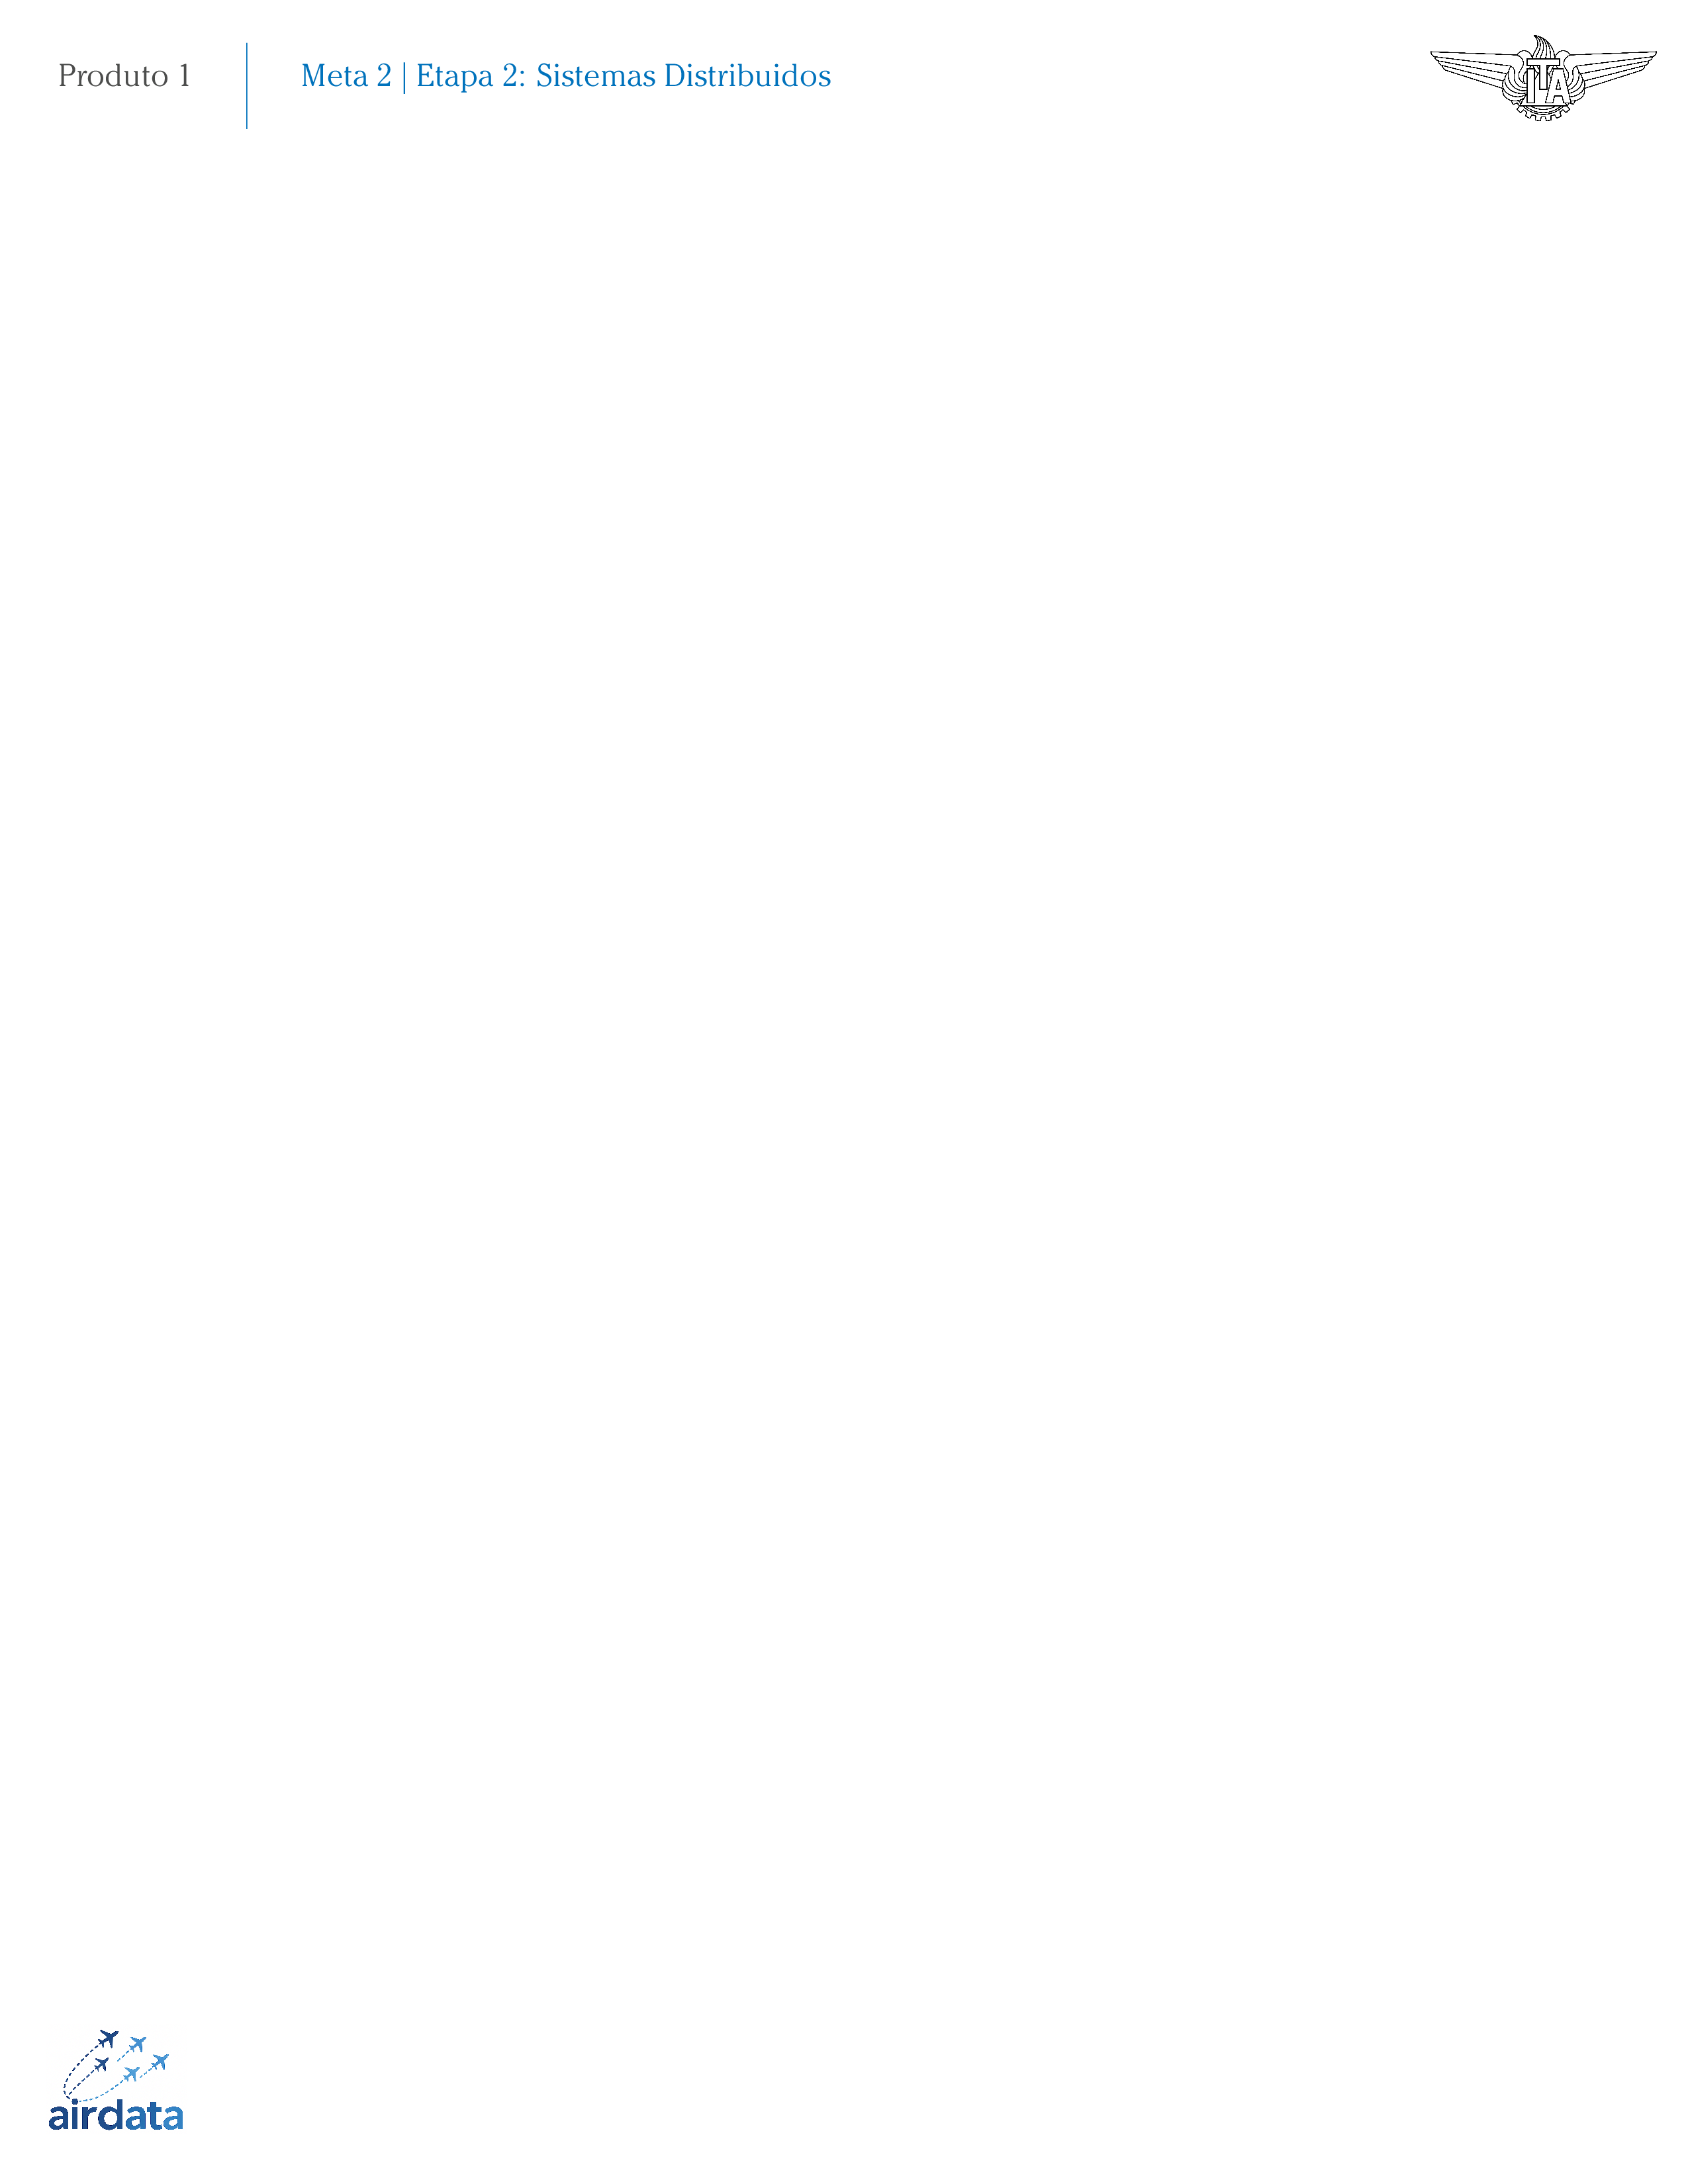
\includegraphics[width=\paperwidth,height=\paperheight]{capas/background.png}%
			\vfill
		}%
	}%
}

% Aplica a imagem de fundo em TODAS as páginas
\AddToShipoutPictureBG{\BackgroundPic}

% settings/pretextualpages.tex
% Define o background exclusivo para páginas pré-textuais

\newenvironment{pretextualblock}
{
	\ClearShipoutPictureBG
	\AddToShipoutPictureBG{
		\put(0,0){
			\parbox[b][\paperheight]{\paperwidth}{%
				
\includegraphics[width=\paperwidth,height=\paperheight]{capas/background_pretex}%
			}
		}
	}
}
{
	\input{settings/background.tex} % Restaura o background padrão
}

\end{verbatim}

Essa ordem é proposital para garantir que os pacotes e estilos sejam carregados antes dos elementos visuais como capa e plano de fundo.

\section{Sugestão de novos capítulos}

Novos arquivos podem ser adicionados à pasta \texttt{caps/} com nomes como \texttt{cap03.tex}, \texttt{cap04.tex}, etc. A inclusão no documento é feita via:

\begin{verbatim}
\chapter{Estrutura do Template}

O template TED ITA-SAC foi organizado de forma modular, para facilitar manutenção, reuso e colaboração entre diferentes autores. A estrutura principal está organizada da seguinte forma:

\section{Visão geral}

\begin{verbatim}
	.
	|- main.tex                 % Arquivo principal (documento raiz)
	|- settings/                % Configurações gerais
	|  |- background.tex        % Marca d’água e fundo
	|  |- coverpage.tex         % Página de capa
	|  |- fonts.tex             % Fonte Cheltenham
	|  |- pretextualpages.tex  % Sumário, listas, elementos iniciais
	|  |- setabnt.tex          % Estilo de citação ABNT
	|  |- setcolor.tex         % Paleta de cores do template
	|  |- setlayout.tex        % Margens, espaçamento, cabeçalho
	|  |- settitles.tex        % Estilo de títulos e capítulos
	|  \_ usepackage.tex       % Pacotes utilizados no projeto
	|- caps/                   % Capítulos do relatório
	|  |- cap00.tex            % Introdução
	|  |- cap01.tex            % Conteúdo específico
	|  \_ etc.
	|- siglas/                 % (Opcional) Siglas, glossários
	|- refs/                   % (Opcional) Arquivos .bib
	\_ Makefile                % Automação de compilação
\end{verbatim}


\section{Função de cada componente}

\begin{itemize}
    \item \texttt{main.tex}: ponto de entrada do projeto. Controla a ordem dos elementos.
    \item \texttt{settings/}: conjunto de arquivos para configurar todos os aspectos do template.
    \item \texttt{caps/}: contém os capítulos do relatório (modularizados).
    \item \texttt{siglas/}: pasta destinada ao glossário e acrônimos, caso ativado.
    \item \texttt{refs/}: local sugerido para o arquivo de bibliografia (\texttt{.bib}).
    \item \texttt{Makefile}: automatiza as etapas de compilação (XeLaTeX + BibTeX + Glossário).
\end{itemize}

\section{Ordem de carregamento no \texttt{main.tex}}

O arquivo \texttt{main.tex} importa os componentes da seguinte forma:

\begin{verbatim}
\input{settings/usepackage.tex}
\input{settings/setabnt.tex}
\input{settings/setlayout.tex}
\input{settings/fonts.tex}
\input{settings/setcolor.tex}
\input{settings/settitles.tex}
\input{settings/coverpage.tex}
\input{settings/background.tex}
\input{settings/pretextualpages.tex}
\end{verbatim}

Essa ordem é proposital para garantir que os pacotes e estilos sejam carregados antes dos elementos visuais como capa e plano de fundo.

\section{Sugestão de novos capítulos}

Novos arquivos podem ser adicionados à pasta \texttt{caps/} com nomes como \texttt{cap03.tex}, \texttt{cap04.tex}, etc. A inclusão no documento é feita via:

\begin{verbatim}
\input{caps/cap03.tex}
\end{verbatim}

Recomenda-se utilizar comandos \verb|\chapter| dentro de cada arquivo, para manter a consistência da numeração.



\end{verbatim}

Recomenda-se utilizar comandos \verb|\chapter| dentro de cada arquivo, para manter a consistência da numeração.



\end{verbatim}

Recomenda-se utilizar comandos \verb|\chapter| dentro de cada arquivo, para manter a consistência da numeração.



	
	
	\cleardoublepage
	\pagestyle{plain}
	\chapter{Fontes e Tipografia}

A identidade visual do template TED ITA-SAC adota a tipografia Cheltenham ITC Pro como fonte principal. Essa fonte deve estar instalada no sistema operacional, pois sua ativação depende do pacote fontspec, que só funciona com o compilador XeLaTeX.

\section{Configuração no template}

A configuração da fonte é realizada no arquivo:

settings/fonts.tex

Seu conteúdo básico é:

usepackage{fontspec}
setmainfont[
Path = ./fonts/,
Extension = .otf,
UprightFont = *-Roman,
BoldFont = *-Bold,
ItalicFont = *-Italic,
BoldItalicFont = *-BoldItalic
]{Cheltenham}

Observação: a fonte precisa estar disponível no diretório "fonts/" ou instalada no sistema com esse mesmo nome (Cheltenham).

\section{Instalação da fonte}

Em sistemas Linux:
- Crie o diretório de fontes e atualize o cache:

mkdir -p ~/.fonts/cheltenham  
cp *.otf ~/.fonts/cheltenham/  
fc-cache -fv

Em sistemas Windows:
- Clique com o botão direito nos arquivos .otf e selecione "Instalar".

Em sistemas macOS:
- Clique duas vezes nos arquivos .otf e clique em "Instalar fonte".

\section{Compilador: XeLaTeX obrigatório}

A compilação deve ser feita exclusivamente com o compilador xelatex, pois os pacotes fontspec e polyglossia (ou babel com suporte a unicode) exigem esse motor para ativar fontes do sistema ou arquivos OpenType.

Para compilar no terminal:

xelatex main.tex

Ou via Makefile:

make

\section{Mensagens de erro comuns}

- Font not found: a fonte não está instalada ou o nome está incorreto.
- Missing character: There is no...: está sendo usado um caractere Unicode que a fonte atual não suporta.
- Package fontspec Error: The font "Cheltenham" cannot be found: verifique se os arquivos .otf estão acessíveis no caminho correto.

\section{Sugestões para fallback}

Se não desejar usar Cheltenham, é possível substituir por outra fonte compatível. Exemplos:

setmainfont{TeX Gyre Pagella}  
ou  
setmainfont{Times New Roman}

Importante: fontes padrão como Times ou Latin Modern não representam a identidade visual original do projeto TED ITA-SAC.

	
	
	\cleardoublepage
	\pagestyle{plain}
	\chapter{Layout e Margens}

O controle da geometria da página no template TED ITA-SAC é feito por meio do arquivo:

\begin{verbatim}
	settings/setlayout.tex
\end{verbatim}

Esse arquivo configura as margens, espaçamentos, cabeçalhos e rodapés, garantindo uma apresentação institucionalmente adequada e confortável para leitura.

\section{Configuração de margens}

O pacote \texttt{geometry} é utilizado para definir as dimensões da página:

\begin{verbatim}
	\usepackage[
	a4paper,
	left=3cm,
	right=2.5cm,
	top=3cm,
	bottom=2.5cm,
	headheight=16pt,
	includeheadfoot
	]{geometry}
\end{verbatim}

Essas medidas foram adotadas com base em boas práticas de editoração técnica e podem ser ajustadas conforme a necessidade.

\section{Espaçamento entre linhas}

O espaçamento é controlado por:

\begin{verbatim}
	\linespread{1.25}
\end{verbatim}

O valor `1.25` representa um espaçamento levemente expandido (equivalente a 1,5 linhas no Word). Esse valor proporciona boa legibilidade sem comprometer a economia de páginas.

\section{Cabeçalhos e rodapés}

O pacote \texttt{fancyhdr} é utilizado para personalizar cabeçalhos e rodapés:

\begin{verbatim}
	\usepackage{fancyhdr}
	\pagestyle{fancy}
	\fancyhf{}
	\fancyhead[R]{\thepage}
	\fancyhead[L]{\slshape \nouppercase{\leftmark}}
	\renewcommand{\headrulewidth}{0.4pt}
\end{verbatim}

Com essa configuração:

\begin{itemize}
	\item O número da página aparece no canto superior direito;
	\item O título do capítulo aparece no canto superior esquerdo;
	\item A linha divisória do cabeçalho é ativada;
	\item O rodapé permanece vazio.
\end{itemize}

\section{Outros ajustes úteis}

Você pode adicionar a data ou título do projeto ao rodapé, exemplo:

\begin{verbatim}
	\fancyfoot[C]{Projeto TED ITA-SAC}
\end{verbatim}

Para capítulos específicos com layout limpo (como capa ou versão), o comando abaixo pode ser usado:

\begin{verbatim}
	\thispagestyle{empty}
\end{verbatim}

\section{Sugestão de personalização}

Para suprimir o título do capítulo nos cabeçalhos de páginas pares e manter somente o número da página, use:

\begin{verbatim}
	\fancyhead[L]{}
	\fancyhead[R]{\thepage}
\end{verbatim}

Ou, para remover tudo:

\begin{verbatim}
	\pagestyle{empty}
\end{verbatim}


	
	
	\cleardoublepage
	\pagestyle{plain}
	\chapter{Paleta de Cores e Estilo Visual}

A padronização das cores é essencial para manter a identidade visual do projeto TED ITA-SAC. Este capítulo apresenta a paleta cromática adotada para representar a Coordenação Geral, as Metas e as respectivas Etapas.

\section{Visualização da paleta de cores}

A imagem a seguir apresenta a estrutura da paleta de cores, organizada por metas e etapas.

Arquivo da imagem: images/paleta\_cores.png


Legenda: Códigos de cor utilizados no projeto por meta e etapa.


\section{Definição das cores no template}

As cores são definidas no arquivo:

settings/setcolor.tex

Dentro desse arquivo, as cores são registradas com o comando definecolor. Exemplo:

definecolor{meta1etapa4}{HTML}{2b61ae}

Importante: não utilize o comando usepackage{xcolor} dentro de setcolor.tex. Esse pacote já deve estar carregado no arquivo settings/usepackage.tex.

\section{Exemplo de uso no texto}

Para aplicar uma cor ao texto, por exemplo na Etapa 1 da Meta 2:

{color{meta2etapa1} Etapa 1 da Meta 2}

Para destacar uma frase com fundo colorido:

colorbox{meta1etapa4}{parbox de largura reduzida com o texto: "Texto destacado na cor da Etapa 4 da Meta 1."}

Essa caixa deve ser compacta (recomenda-se usar largura de 40% a 50% da linha para evitar que ultrapasse a margem do documento).

\section{Cuidados no uso das cores}

- Evite usar cores com baixo contraste entre fundo e texto.
- Utilize apenas as cores registradas em settings/setcolor.tex.
- Em documentos entregues oficialmente, utilize na capa a cor institucional que corresponde à etapa do projeto, conforme orientação da Coordenação Geral.

	
	
	\cleardoublepage
	\pagestyle{plain}
	\chapter{Estilo de Títulos e Numeração}

A identidade visual dos títulos (capítulos, seções e subseções) é configurada por meio do arquivo:

\begin{verbatim}
	settings/settitles.tex
\end{verbatim}

Esse arquivo utiliza o pacote `titlesec` para modificar o estilo padrão do LaTeX e aplicar:

\begin{itemize}
	\item Fontes com peso e caixa específicos;
	\item Controle de espaçamentos verticais;
	\item Numeração estilizada;
	\item Alinhamento e cor.
\end{itemize}

\section{Títulos de capítulo}

Exemplo de configuração para o comando \verb|\chapter|:

\begin{verbatim}
	\titleformat{\chapter}[display]
	{\normalfont\bfseries\Huge}
	{\chaptername\ \thechapter}
	{1ex}
	{\vspace{0.5ex}}
	\titlespacing*{\chapter}{0pt}{-10pt}{20pt}
\end{verbatim}

Explicação dos parâmetros:

\begin{itemize}
	\item Usa a palavra "Capítulo" seguida do número: \verb|\chaptername \thechapter|;
	\item \verb|\Huge| aumenta o tamanho da fonte do título;
	\item Os espaçamentos antes e depois do título são definidos por \verb|\titlespacing|;
	\item A formatação usa negrito (\verb|\bfseries|) e fonte normal (\verb|\normalfont|).
\end{itemize}

\section{Títulos de seção e subseção}

Exemplo para o comando \verb|\section|:

\begin{verbatim}
	\titleformat{\section}
	{\normalfont\bfseries\Large}
	{\thesection}{1em}{}
	\titlespacing*{\section}{0pt}{2ex plus 1ex}{1ex}
\end{verbatim}

Exemplo para o comando \verb|\subsection|:

\begin{verbatim}
	\titleformat{\subsection}
	{\normalfont\itshape\large}
	{\thesubsection}{1em}{}
\end{verbatim}

Esses estilos mantêm a hierarquia visual clara e consistente entre os níveis de título.

\section{Numeração de títulos}

A numeração automática é gerada com os comandos \verb|\thesection| e \verb|\thesubsection|.

Para remover a numeração de títulos:

\begin{verbatim}
	\setcounter{secnumdepth}{0}
\end{verbatim}

Ou, para seções específicas, é possível redefinir o estilo com:

\begin{verbatim}
	\titleformat{\section}[block]
	{\normalfont\bfseries}{}{0pt}{}
\end{verbatim}

\section{Recomendações}

\begin{itemize}
	\item Use sempre espaçamentos verticais consistentes antes e depois dos títulos;
	\item Evite o uso de letras maiúsculas em todos os títulos;
	\item Alinhe o estilo dos títulos com o restante da identidade visual do projeto;
	\item Edite o arquivo `settings/settitles.tex` para ajustar todos os estilos de forma centralizada.
\end{itemize}

	
	\cleardoublepage
	\pagestyle{plain}
	\chapter{Capa e Plano de Fundo}

O template TED ITA-SAC utiliza uma capa institucional personalizada e uma marca d’água como plano de fundo nas páginas internas. Ambos os elementos foram desenvolvidos com identidade visual própria e integrados ao sistema LaTeX.

\section{Origem dos elementos gráficos}

As artes da capa e da marca d’água foram criadas na plataforma Canva. Estão disponíveis para edição e exportação no seguinte link :


A partir desse link, é possível:

- Alterar o título, logotipos ou datas na capa;
- Exportar o plano de fundo como imagem PNG ou PDF;
- Garantir a padronização gráfica do projeto TED ITA-SAC.

\section{Configuração da capa}

A capa é definida no arquivo:

settings/coverpage.tex

Exemplo de estrutura típica:

(begin titlepage)  
(begin center)  
(vspace de 4 cm)  
Título do Documento - fonte grande e negrito  
(vspace de 2 cm)  
Projeto TED ITA-SAC  
Rodapé com ITA, São José dos Campos, ano  
(end center)  
(end titlepage)


Esse arquivo pode ser ajustado para inserir novos títulos, autores, datas ou versões.

\section{Configuração do plano de fundo (marca d’água)}

O plano de fundo é definido no arquivo:

settings/background.tex

Utiliza o pacote "background" com estrutura semelhante a:

usepackage{background}  
backgroundsetup{  
	scale = 1,  
	angle = 0,  
	opacity = 0.07,  
	contents = {imagem de fundo no tamanho da página}  
}

Importante: a imagem chamada background.png deve estar presente no diretório correto.

\section{Dicas de uso e personalização}

- Para remover o fundo em páginas específicas, como a capa, use:  
backgroundsetup{contents={}}

- O fundo pode ser trocado por outra imagem com o mesmo formato;
- A opacidade pode ser ajustada com o parâmetro "opacity";
- Recomenda-se uma imagem com resolução mínima de 150 DPI.

\section{Cores na capa}

A arte da capa criada no Canva inclui uma barra inferior colorida. Essa barra deve utilizar a cor correspondente à etapa do projeto, conforme a paleta oficial (ver Capítulo 6).

Recomendação: cada entrega (relatório técnico, documento ou produto) deve seguir a cor indicada para sua etapa. Isso garante:

- Identificação clara da etapa;
- Padronização visual entre os documentos;
- Coerência com os relatórios enviados ao BNDES.

Exemplo: um relatório da Etapa 4 da Meta 1 deve utilizar a cor meta1etapa4, conforme definida no arquivo settings/setcolor.tex.

	
	\cleardoublepage
	\pagestyle{plain}
	\chapter{Elementos Pré-textuais}

O template TED ITA-SAC inclui uma estrutura pré-definida para os elementos obrigatórios antes do conteúdo técnico. Essa estrutura é configurada no arquivo:

\begin{verbatim}
	settings/pretextualpages.tex
\end{verbatim}

\section{Elementos incluídos}

Por padrão, o arquivo ativa os seguintes componentes:

\begin{itemize}
	\item Sumário (comando \texttt{\textbackslash tableofcontents});
	\item Lista de figuras (comando \texttt{\textbackslash listoffigures});
	\item Lista de tabelas (comando \texttt{\textbackslash listoftables});
	\item Página de controle de versão (opcional);
	\item Marca d’água (ativada no fundo de cada página).
\end{itemize}

\section{Sumário e listas}

A geração do sumário e das listas é automática, com base nos comandos \verb|\chapter|, \verb|\section|, \verb|\caption| e similares.

Para incluir os elementos, basta inserir no arquivo principal \texttt{main.tex}:

\begin{verbatim}
	% settings/pretextualpages.tex
% Define o background exclusivo para páginas pré-textuais

\newenvironment{pretextualblock}
{
	\ClearShipoutPictureBG
	\AddToShipoutPictureBG{
		\put(0,0){
			\parbox[b][\paperheight]{\paperwidth}{%
				
\includegraphics[width=\paperwidth,height=\paperheight]{capas/background_pretex}%
			}
		}
	}
}
{
	% settings/background.tex
% --- Imagem de fundo em todas as páginas ---

% Comando seguro para definir a imagem de fundo
\providecommand\BackgroundPic{%
	\put(0,0){%
		\parbox[b][\paperheight]{\paperwidth}{%
			\vfill
			\centering
			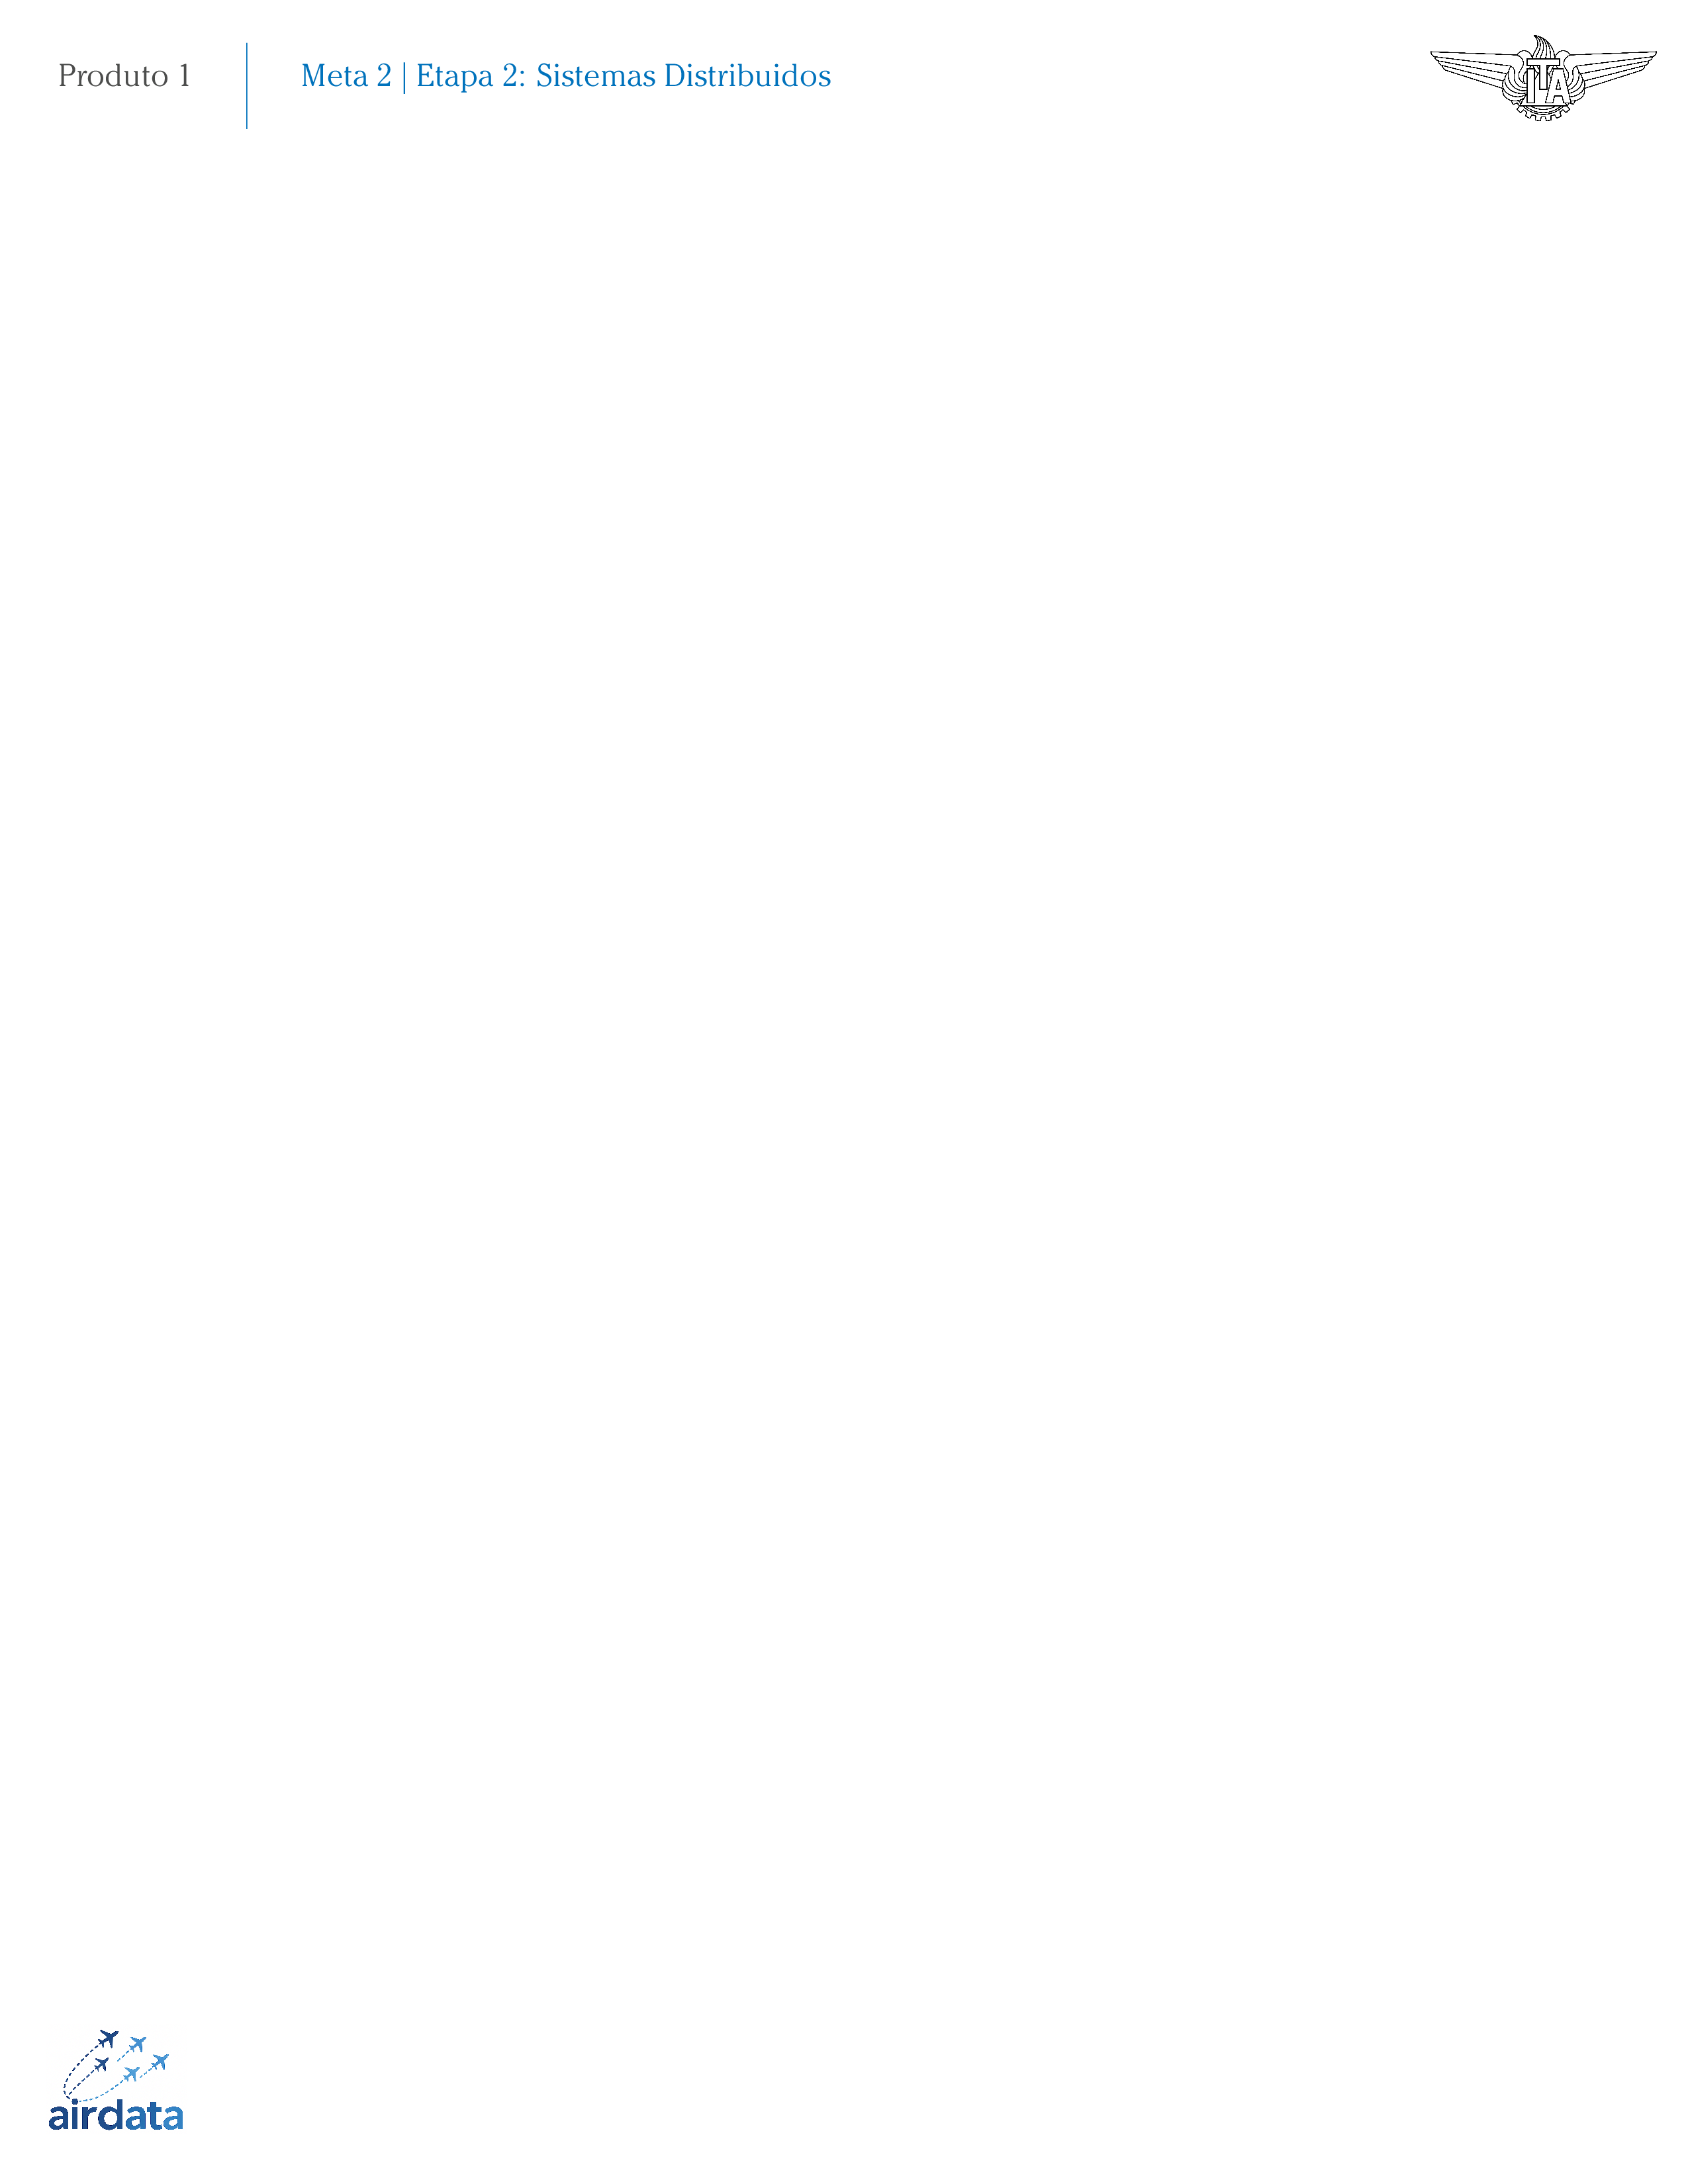
\includegraphics[width=\paperwidth,height=\paperheight]{capas/background.png}%
			\vfill
		}%
	}%
}

% Aplica a imagem de fundo em TODAS as páginas
\AddToShipoutPictureBG{\BackgroundPic}
 % Restaura o background padrão
}

\end{verbatim}

E no conteúdo desse arquivo, deve constar:

\begin{verbatim}
	\tableofcontents
	\listoffigures
	\listoftables
	\cleardoublepage
\end{verbatim}

\section{Folha de versão}

A folha de controle de versão pode ser incluída antes do conteúdo técnico com:

\begin{verbatim}
	\input{caps/cap_controleversao.tex}
\end{verbatim}

Esse arquivo pode conter uma tabela com histórico de alterações, como:

\begin{center}
	\begin{tabular}{|c|c|c|l|}
		\hline
		Versão & Data & Responsável & Descrição \\
		\hline
		1.0 & 01/08/2025 & Coordenação & Documento inicial \\
		1.1 & 05/08/2025 & Revisores & Correções ortográficas \\
		\hline
	\end{tabular}
\end{center}

\section{Numeração romana}

Antes do início do conteúdo principal, a numeração é configurada em algarismos romanos:

\begin{verbatim}
	\pagenumbering{roman}
	\pagestyle{empty}
\end{verbatim}

Essa numeração é trocada para arábica ao iniciar o corpo do relatório:

\begin{verbatim}
	\cleardoublepage
	\pagenumbering{arabic}
\end{verbatim}

\section{Boas práticas}

\begin{itemize}
	\item Mantenha a ordem: capa $\rightarrow$ controle de versão $\rightarrow$ sumário/listas $\rightarrow$ conteúdo;
	\item Use sempre \verb|\cleardoublepage| entre seções principais para garantir início em página ímpar;
	\item Atualize a folha de versão a cada entrega formal do projeto.
\end{itemize}

	
	
		
	\cleardoublepage
	\pagestyle{plain}
	\chapter{Referências e Estilo ABNT}

O template TED ITA-SAC utiliza o estilo de citações e referências conforme as normas da ABNT, implementado via o pacote abntex2cite em conjunto com o BibTeX. Essa abordagem permite o uso padronizado de citações autor-data e a geração automática da lista de referências.

\section{Configuração do estilo}

A configuração está centralizada no arquivo:

settings/setabnt.tex

O arquivo de referências utilizado deve estar em formato BibTeX (.bib), preferencialmente localizado em:

refs/referencias.bib

\section{Exemplos de citações reais}

Abaixo estão exemplos práticos utilizando as chaves presentes no arquivo `.bib`:

Segundo \citeonline{murca2020characterizing}, a análise do desempenho do espaço aéreo brasileiro pode ser realizada por meio de dados de trajetória.

Estudos sobre priorização de investimentos em aeródromos da aviação geral são apresentados em \cite{caetano2022criteria}.

A ineficiência vertical em procedimentos de descida foi discutida por \cite{szenczuk2021causalvertical} sob uma abordagem causal.

\section{Citação múltipla}

Também é possível citar múltiplas referências no mesmo trecho:

Diversos autores têm contribuído para o tema da infraestrutura e operação aérea no Brasil \cite{murca2020characterizing, caetano2022criteria, szenczuk2021causalvertical}.


\section{Compilação com BibTeX}

A sequência recomendada para compilar e gerar corretamente as referências é:

1. Rodar `xelatex main.tex`  
2. Rodar `bibtex main.aux`  
3. Rodar `xelatex main.tex` duas vezes

Se estiver usando o Makefile do template, isso já está automatizado com:

make

\section{Observações}

- As chaves entre chaves `{}` devem coincidir exatamente com as do arquivo `.bib`.
- A ordem de chamada das referências será ajustada automaticamente com base na ordem de citação no texto.
- Referências não citadas no texto não aparecerão na bibliografia final.

	
	
			
	\cleardoublepage
	\pagestyle{plain}
	\chapter{Siglas e Glossário}

O template TED ITA-SAC oferece suporte à criação automática de listas de siglas e de termos técnicos por meio do pacote \texttt{glossaries-extra}. Ele permite organizar e exibir os acrônimos usados ao longo do documento, de forma consistente e padronizada.

\section{Definição das siglas}

As siglas são definidas no arquivo: cap\_siglas.tex


\section{Uso no corpo do texto}

As siglas podem ser usadas normalmente com o comando \verb|\gls|. Veja os exemplos a seguir:

\begin{itemize}
	\item A \gls{icao} é o órgão responsável por padronizar normas internacionais de aviação;
	\item O \gls{ganp} estabelece a visão de longo prazo para o desenvolvimento do \gls{atm};
	\item Iniciativas como o \gls{utmx} buscam integrar soluções de mobilidade aérea urbana.
\end{itemize}

Na primeira ocorrência de cada sigla, será exibido o significado completo seguido da abreviação. Nas ocorrências seguintes, apenas a abreviação.


	
	\bibliographystyle{abntex2-alf}
	\bibliography{abntex2-options,refs/referencias}

	
	
\end{document}
